%%%%%%%%%%%%%%%%%%%%%%%%%%%%%%%%%%%%%%%%%%%%%%%%%%%%%%%%%%
%   Autoren:
%   Prof. Dr. Bernhard Drabant
%   Prof. Dr. Dennis Pfisterer
%   Prof. Dr. Julian Reichwald
%%%%%%%%%%%%%%%%%%%%%%%%%%%%%%%%%%%%%%%%%%%%%%%%%%%%%%%%%%

%%%%%%%%%%%%%%%%%%%%%%%%%%%%%%%%%%%%%%%%%%%%%%%%%%%%%%%%%%
%	ANLEITUNG:
%   1. Ersetzen Sie firmenlogo.jpg im Verzeichnis img
%   2. Passen Sie alle Stellen im Dokument an, die mit
%      @stud
%      markiert sind
%%%%%%%%%%%%%%%%%%%%%%%%%%%%%%%%%%%%%%%%%%%%%%%%%%%%%%%%%%

%%%%%%%%%%%%%%%%%%%%%%%%%%%%%%%%%%%%%%%%%%%%%%%%%%%%%%%%%%
%	ACHTUNG:
%   Für das Erstellen des Literaturverzeichnisses wird das
%   modernere Paket biblatex in Kombination mit biber
%   verwendet - nicht mehr das ältere Paket BibTex!
%
%   Bitte stellen Sie Ihre TeX-Umgebung entsprechend ein (z.B. TeXStudio):
%   Einstellungen --> Erzeugen --> Standard Bibliographieprogramm: biber
%%%%%%%%%%%%%%%%%%%%%%%%%%%%%%%%%%%%%%%%%%%%%%%%%%%%%%%%%%

\documentclass[fontsize=12pt,BCOR=5mm,DIV=12,parskip=half,listof=totoc,
               paper=a4,toc=bibliography,pointlessnumbers]{scrreprt}

\usepackage[utf8]{inputenc}

%% LANGUAGE SETTINGS
%
% @stud: Sprache ggf. anpassen
%
%\usepackage[ngerman]{babel} 	        % german language
%\usepackage[german=quotes]{csquotes} 	% correct quoting using \enquote{}
\usepackage[english]{babel}          % english language
\usepackage{csquotes} 	              % correct quoting using \enquote{}

%%%%%%%%%%%%%
%% ZITIERSTIL
%%%%%%%%%%%%%
%
% @stud: Zitierstil in package biblatex unten wählen
%
% NUMERIC Style - e. g. [12]
% style=numeric
%
% IEEE Style - numeric kind of style
% style=ieee
%
% ALPHABETIC Style - e. g. [AB12]
% style=alphabetic
%
% HARVARD Style
% style=apa
%
% CHICAGO Style
% style=authoryear
%
% Position des Zitats:
%
% autocite=inline
%
% (!!) FOOTNOTE POSITION NOT RECOMMENDED IN MINT DOMAIN:
% autocite=footnote
%
\usepackage[backend=biber, autocite=inline, style=apa]{biblatex}
\usepackage{makeidx}                  % allows index generation
\usepackage{listings}	                %Format Listings properly
\usepackage{lipsum}                   % Blindtext
\usepackage{graphicx}                 % use various graphics formats
\usepackage[german]{varioref}         % nicer references \vref
\usepackage{caption}	                % better Captions
\usepackage{booktabs}                 % nicer Tabs
\usepackage[hidelinks=true]{hyperref} % keine roten Markierungen bei Links
\usepackage{fnpct}                    % Correct superscripts
\usepackage{calc}                     % Used for extra space below footsepline, in particular
\usepackage{array}
\usepackage{acronym}
\usepackage{algorithm}
\usepackage{algpseudocode}
\usepackage{setspace}
\usepackage{tocloft}
\usepackage[T1]{fontenc}
\usepackage{multirow}
\usepackage{amsmath}
\usepackage{amssymb}
\usepackage{rotating}

% Definitionen und Commands
\newcommand{\indextype}{numeric}
\newcommand{\abs}{\par\vskip 0.2cm\goodbreak\noindent}
\newcommand{\nl}{\par\noindent}
\newcommand{\mcl}[1]{\mathcal{#1}}
\newcommand{\nowrite}[1]{}
\newcommand{\NN}{{\mathbb N}}
\newcommand{\imagedir}{img}
\newcommand{\TitelDerArbeit}[1]{\def\DerTitelDerArbeit{#1}\hypersetup{pdftitle={#1}}}
\newcommand{\AutorDerArbeit}[1]{\def\DerAutorDerArbeit{#1}\hypersetup{pdfauthor={#1}}}
\newcommand{\Firma}[1]{\def\DerNameDerFirma{#1}}
\newcommand{\Kurs}[1]{\def\DieKursbezeichnung{#1}}
\newcommand{\Abteilung}[1]{\def\DerNameDerAbteilung{#1}}
\newcommand{\Studiengangsleiter}[1]{\def\DerStudiengangsleiter{#1}}
\newcommand{\WissBetreuer}[1]{\def\DerWissBetreuer{#1}}
\newcommand{\FirmenBetreuer}[1]{\def\DerFirmenBetreuer{#1}}
\newcommand{\Bearbeitungszeitraum}[1]{\def\DerBearbeitungszeitraum{#1}}
\newcommand{\Abgabedatum}[1]{\def\DasAbgabedatum{#1}}
\newcommand{\Matrikelnummer}[1]{\def\DieMatrikelnummer{#1}}
\newcommand{\Studienrichtung}[1]{\def\DieStudienrichtung{#1}}
\newcommand{\ArtDerArbeit}[1]{\def\DieArtDerArbeit{#1}}
\newcommand{\Literaturverzeichnis}{Literaturverzeichnis}

% Page Layout
\oddsidemargin=0mm
\evensidemargin=0mm
\textwidth=159mm
\topmargin=-18mm
\headsep=10mm
\textheight=251mm
\footheight=15mm

\makeindex

%%%%%%%%%%%%%%%%%%%%%%%%%%%%%%%%%%%
% LITERATURVERZEICHNIS
% @stud: Literaturverzeichnis in Datei bibliography.bib anpassen.
%
% [Alternative zu Verwendung von \initializeBibliography: Citavi ... (dazu eigenes LaTex Coding verwenden)]
%
\addbibresource{bibliography.bib}
\DefineBibliographyStrings{ngerman}{andothers = {{et\,al\adddot}},}

% Elementare Konfigurationen und Definitionen werden geladen
% @stud: gegebenenfalls anpassen
%
% !TEX root =  master.tex

%%%%%%%%%%%%%%%%%%%%%%%%%%%%%%%%%%%%%%%%%%%%%%%%%%%%%%%%%%%%%%%%%%
%	ANLEITUNG:
% Passen Sie gegebenenfalls alle Stellen im Dokument an, die mit
% @stud
% markiert sind.
%%%%%%%%%%%%%%%%%%%%%%%%%%%%%%%%%%%%%%%%%%%%%%%%%%%%%%%%%%%%%%%%%%

%%
%% @stud
%%
%% LANGUAGE SETTINGS
% \usepackage[ngerman]{babel} 	        % german language
% \usepackage[german=quotes]{csquotes} 	% correct quoting using \enquote{}
\usepackage[english]{babel}          % english language
\usepackage{csquotes} 	              % correct quoting using \enquote{}

\usepackage{makeidx}                  % allows index generation
\usepackage{listings}	                %Format Listings properly
\usepackage{lipsum}                   % Blindtext
\usepackage{graphicx}                 % use various graphics formats
\usepackage[german]{varioref}         % nicer references \vref
\usepackage{caption}	                % better Captions
\usepackage{booktabs}                 % nicer Tabs
\usepackage[hidelinks=true]{hyperref} % keine roten Markierungen bei Links
\usepackage{fnpct}                    % Correct superscripts
\usepackage{calc}                     % Used for extra space below footsepline, in particular
\usepackage{array}
\usepackage{acronym}
\usepackage{algorithm}
\usepackage{algpseudocode}
\usepackage{setspace}
\usepackage{tocloft}

%% Schriftarten- und Zeichenpakete
\usepackage[T1]{fontenc}
\usepackage[utf8]{inputenc}

%%
%% @stud
%%
%%	FONT SELECTION: Schriftarten und Schriftfamilie
%%%%%%%%%%%%%
%% SCHRIFTART
%%%%%%%%%%%%%
% 0) without decomment: normal font families
% ...
% 1) Latin Modern
%\usepackage{lmodern}
% 2) Times
%\usepackage{mathptmx}
% 3) Helvetica
%\usepackage[scaled=.92]{helvet}
%%%%%%%%%%%%%%%%%%
%%	SCHRIFTFAMILIE
%%%%%%%%%%%%%%%%%%
% ohne Serifen
\renewcommand*{\familydefault}{\sfdefault}
\addtokomafont{disposition}{\sffamily}
%
% mit Serifen
%\renewcommand*{\familydefault}{\rmdefault}
%\addtokomafont{disposition}{\rmfamily}
%
% Typewriter
%\renewcommand*{\familydefault}{\ttdefault}
%\addtokomafont{disposition}{\ttfamily}

%%
%% @stud
%%
%% Uncomment the following lines to support hard URL breaks in bibliography
%\apptocmd{\UrlBreaks}{\do\f\do\m}{}{}
%\setcounter{biburllcpenalty}{9000}% Kleinbuchstaben
%\setcounter{biburlucpenalty}{9000}% Großbuchstaben

%%
%% @stud
%%
%% FOOTNOTES: Count footnotes over chapters
%% \counterwithout{footnote}{chapter}

%	ACRONYMS
\makeatletter
\@ifpackagelater{acronym}{2015/03/20}
{\renewcommand*{\aclabelfont}[1]{\textbf{{\acsfont{#1}}}}}{}
\makeatother

%	LISTINGS
% @stud: ggf. Namen/Text anpassen (englisch)
\renewcommand{\lstlistingname}{Source Code}
\renewcommand{\lstlistlistingname}{List of Source Code}
\lstset{numbers=left,
	numberstyle=\tiny,
	captionpos=b,
	basicstyle=\ttfamily\small}

%	ALGORITHMS
% @stud: ggf. Namen/Text anpassen (englisch)
\renewcommand{\listalgorithmname}{Algorithmenverzeichnis}
\floatname{algorithm}{Algorithmus}

%	PAGE HEADER / FOOTER
%	Warning: There are some redefinitions throughout the master.tex-file!  DON'T CHANGE THESE REDEFINITIONS!
\RequirePackage[automark]{scrlayer-scrpage}
%alternatively with separation lines: \RequirePackage[automark,headsepline,footsepline]{scrlayer-scrpage}

\renewcommand{\chaptermarkformat}{}
\RedeclareSectionCommand[beforeskip=0pt]{chapter}
\clearpairofpagestyles

%\ifoot[\rule{0pt}{\ht\strutbox+\dp\strutbox}DHBW Mannheim]{\rule{0pt}{\ht\strutbox+\dp\strutbox}DHBW Mannheim}
\ofoot[\rule{0pt}{\ht\strutbox+\dp\strutbox}\pagemark]{\rule{0pt}{\ht\strutbox+\dp\strutbox}\pagemark}
\ohead{\headmark}

% \newcommand{\TitelDerArbeit}[1]{\def\DerTitelDerArbeit{#1}\hypersetup{pdftitle={#1}}}
% \newcommand{\AutorDerArbeit}[1]{\def\DerAutorDerArbeit{#1}\hypersetup{pdfauthor={#1}}}
% \newcommand{\Firma}[1]{\def\DerNameDerFirma{#1}}
% \newcommand{\Kurs}[1]{\def\DieKursbezeichnung{#1}}
% \newcommand{\Abteilung}[1]{\def\DerNameDerAbteilung{#1}}
% \newcommand{\Studiengangsleiter}[1]{\def\DerStudiengangsleiter{#1}}
% \newcommand{\WissBetreuer}[1]{\def\DerWissBetreuer{#1}}
% \newcommand{\FirmenBetreuer}[1]{\def\DerFirmenBetreuer{#1}}
% \newcommand{\Bearbeitungszeitraum}[1]{\def\DerBearbeitungszeitraum{#1}}
% \newcommand{\Abgabedatum}[1]{\def\DasAbgabedatum{#1}}
% \newcommand{\Matrikelnummer}[1]{\def\DieMatrikelnummer{#1}}
% \newcommand{\Studienrichtung}[1]{\def\DieStudienrichtung{#1}}
% \newcommand{\ArtDerArbeit}[1]{\def\DieArtDerArbeit{#1}}
% \newcommand{\Literaturverzeichnis}{Literaturverzeichnis}

\newcommand{\settingBibFootnoteCite}{
	\setlength{\bibparsep}{\parskip}		  % Add some space between biblatex entries in the bibliography
	\addbibresource{bibliography.bib}	    % Add file bibliography.bib as biblatex resource
	\DefineBibliographyStrings{ngerman}{andothers = {{et\,al\adddot}},}
}

\newcommand{\setTitlepage}{
	% !TEX root =  master.tex
% @stud: ggf. Namen/Text anpassen (englisch)
\begin{titlepage}
\begin{minipage}{\textwidth}
		\vspace{-2cm}
		% \noindent 
\includegraphics[scale=0.25]{\imagedir/firmenlogo.jpeg} 
    \begin{center}
        
\includegraphics{\imagedir/logo.jpeg}
    \end{center}
\end{minipage}
\vspace{1em}
%\sffamily
\begin{center}
	{\textsf{\large Duale Hochschule Baden-W\"urttemberg Mannheim}}\\[4em]
	{\textsf{\textbf{Advanced Machine Learning}}}\\[6mm]
	{\textsf{\textbf{\Large{}\DerTitelDerArbeit}}} \\[1.5cm]
	{\textsf{\textbf{\large{}Studiengang Wirtschaftsinformatik}}\\[6mm]
	\textsf{\textbf{Studienrichtung \DieStudienrichtung}}}\vspace{10em}
	
	\begin{minipage}{\textwidth}
		\begin{tabbing}
		Wissenschaftliche(r) Betreuer(in): \hspace{0.25cm}\=\kill
		Verfasser: \> \DerAutorDerArbeit \\[1.5mm]
		Matrikelnummern: \> 3465546, 9467152, 9603221 \\[1.5mm]
		% Firma: \> \DerNameDerFirma  \\[1.5mm]
		% Abteilung: \> \DerNameDerAbteilung \\[1.5mm]
		Kurs: \> \DieKursbezeichnung \\[1.5mm]
		Modul: \> Advanced Machine Learning \\[1.5mm]
		Kursleiter: \> \DerStudiengangsleiter \\[1.5mm]
		% Wissenschaftliche(r) Betreuer(in): \> \DerWissBetreuer \\[1.5mm]
		% Firmenbetreuer(in): \> \DerFirmenBetreuer \\[1.5mm]
		Bearbeitungszeitraum: \> \DerBearbeitungszeitraum\\[1.5mm]
%		alternativ:\\[1.5mm]
%		Eingereicht: \> \DasAbgabedatum	
		\end{tabbing}
	\end{minipage}
\end{center}
\end{titlepage}
	\pagenumbering{roman} % Römische Seitennummerierung
	\normalfont
}

\newcommand{\initializeText}{
	\clearpage
	\ihead{\chaptername~\thechapter} % Neue Header-Definition
	\pagenumbering{arabic}           % Arabische Seitenzahlen
}

\newcommand{\initializeBibliography}{
	\ihead{}
	\printbibliography[title=\Literaturverzeichnis]
	\cleardoublepage
}

\newcommand{\initializeAppendix}{
	\appendix
	\ihead{}
	\cftaddtitleline{toc}{chapter}{Appendix}{}
}



% @stud
%
% PERSÖNLICHE ANGABEN (BITTE VOLLSTÄNDIG EINGEBEN zwischen den Klammern: {...})
%
\ArtDerArbeit{Projekt} % "Bachelor" oder "Projekt" wählen
\TitelDerArbeit{Earthquake Forecasting}
\AutorDerArbeit{André Anan Gilbert, Felix Noll, Marc Grün}
\Kurs{WWI 21 DSB}
\Studienrichtung{Data Science}
\Matrikelnummer{3465546}
\Studiengangsleiter{Prof. Dr. Maximilian Scherer} % Kursleiter
\Bearbeitungszeitraum{06.05.2024 - 24.07.2024}
\Abgabedatum{dd.mm.yyyy}

\begin{document}

\setTitlepage

%%%%%%%%%%%%%%%%%%%%%%%%%%%%%%%%%%%
% EHRENWÖRTLICHE ERKLÄRUNG
%
% @stud: ewerkl.tex bearbeiten
%
% % !TEX root =  master.tex
\clearpage
\chapter*{Statutory Declaration}

% Wird die folgende Zeile auskommentiert, erscheint die ehrenwörtliche
% Erklärung im Inhaltsverzeichnis.

% \addcontentsline{toc}{chapter}{Ehrenwörtliche Erklärung}
I herewith declare that I have composed the present thesis with the title ``\textit{\DerTitelDerArbeit}'' myself and without use of any other than the cited sources and aids. Sentences or parts of sentences quoted literally are marked as such; other references with regard to the statement and scope are indicated by full details of the publications concerned.

The thesis in the same or similar form has not been submitted to any examination body and has not been published.

\vspace{3cm}
Place, Date \hfill \DerAutorDerArbeit

% \cleardoublepage
%%%%%%%%%%%%%%%%%%%%%%%%%%%%%%%%%%%

%%%%%%%%%%%%%%%%%%%%%%%%%%%%%%%%%%%
% SPERRVERMERK
%
% @stud: nondisclosurenotice.tex bearbeiten
%
% % !TEX root =  master.tex
\chapter*{Non-Disclosure Notice}

The content of this work may not be made available to people outside of the examination and evaluation process, either as a whole or in part, unless otherwise authorized by the dual partner.

\cleardoublepage

% \cleardoublepage
%%%%%%%%%%%%%%%%%%%%%%%%%%%%%%%%%%%

%%%%%%%%%%%%%%%%%%%%%%%%%%%%%%%%%%%
%	KURZFASSUNG
%
% @stud: acknowledge.tex bearbeiten
%
% % !TEX root =  master.tex
\chapter*{Danksagung}

Hier können Sie eine Danksagung schreiben. 



% \cleardoublepage
%%%%%%%%%%%%%%%%%%%%%%%%%%%%%%%%%%%

%%%%%%%%%%%%%%%%%%%%%%%%%%%%%%%%%%%
% VERZEICHNISSE und ABSTRACT
%
% @stud: ggf. nicht benötigte Verzeichnisse auskommentieren/löschen
%
\tableofcontents
\cleardoublepage

% Abbildungsverzeichnis
\phantomsection
\addcontentsline{toc}{chapter}{\listfigurename}
\listoffigures
\cleardoublepage

%	Tabellenverzeichnis
% \phantomsection
% \addcontentsline{toc}{chapter}{\listtablename}
% \listoftables
% \cleardoublepage

%	Listingsverzeichnis / Quelltextverzeichnis
\lstlistoflistings
\cleardoublepage

% Algorithmenverzeichnis
% \listofalgorithms
% \cleardoublepage

% Abkürzungsverzeichnis
% @stud: acronyms.tex bearbeiten
% !TEX root =  master.tex
\clearpage
\chapter*{Acronyms}	
\addcontentsline{toc}{chapter}{Acronyms}

\begin{acronym}[XXXXXXX]
    \acro{ARIMA}{Autoregressive Integrated Moving Average}
    \acro{EMA}{Exponential Moving Average}
    \acro{FDSN}{International Federation of Digital Seismograph Networks}
    \acro{FFT}{Fast Fourier Transformation}
    \acro{LLM}{Large Language Model}
    \acro{LSTM}{Long Short-Term Memory}
    \acro{MAE}{Mean Absolute Error}
    \acro{MAPE}{Mean Absolute Percentage Error}
    \acro{MSE}{Mean Squared Error}
    \acro{IOT}{Internet of Things}
    \acro{PACF}{Partial Autocorrelation Functions}
    \acro{PCA}{Principal Component Analysis}
    \acro{RMSE}{Root Mean Squared Error}
    \acro{RNNs}{Recurrent Neural Networks}
    \acro{SMA}{Simple Moving Average}
    \acro{USGS}{United States Geological Survey}
\end{acronym}
\cleardoublepage

\onehalfspacing

%	Kurzfassung / Abstract
% @stud: abstract.tex bearbeiten
\chapter*{Abstract}

Earthquakes are a common, yet sometimes catastrophic, phenomenon in our world.
Approximately 2,000 earthquakes with a magnitude of 5 on the Richter scale
occur annually \parencite{welt_erdbeben}. As this threat frequently endangers
many lives, we aim to improve response time and enhance public understanding
of earthquakes, particularly how to act in extreme situations. To achieve this,
we have developed a CatBoost model to forecast the magnitude and depth of
upcoming earthquakes for the 25 most vulnerable regions over the next three days.
Our model achieves a \ac{MSE} of 2.9344, a \ac{RMSE} of 10.3577, and an R2 score
of 0.9495. Additionally, we have developed a \ac{LLM}-powered AI agent,
enabling user interaction with the model results and
providing answers to general questions about earthquakes to improve awareness and
in-depth analysis of potential risks and safety measures. This project contributes
to the field of forecasting research by exemplifying the use case of a categorical
boosted tree model to forecast earthquakes.

\addcontentsline{toc}{chapter}{Abstract}

\cleardoublepage

\initializeText

%%%%%%%%%%%%%%%%%%%%%%%%%%%%%%%%%%%%%%%%%%%%%%%%%%%%%%%%%%%%%%%%%%%%%%%%%%%%%%%%%%%%%%%%%%
% KAPITEL UND ANHÄNGE
%
% @stud:
%   - nicht benötigte: auskommentieren/löschen
%   - neue: bei Bedarf hinzufügen mittels input-Kommando an entsprechender Stelle einfügen
%%%%%%%%%%%%%%%%%%%%%%%%%%%%%%%%%%%%%%%%%%%%%%%%%%%%%%%%%%%%%%%%%%%%%%%%%%%%%%%%%%%%%%%%%%

%%%%%%%%%%%%%%%%%%%%%%%%%%%%%%%%%%%
% KAPITEL
%
% @stud: einzelne Kapitel bearbeiten und eigene Kapitel hier einfügen
%
% Einleitung
% !TEX root =  master.tex

\chapter{Introduction}
Earthquakes are a common phenomenon in our world, with approximately 2,000 earthquakes
of magnitude 5 on the Richter scale occurring annually \parencite{welt_erdbeben}.
While these earthquakes are classified as moderate, they still have the potential
to be deadly and cause significant damage to infrastructure and communities. The
unpredictability of earthquakes poses a considerable challenge to disaster preparedness
and risk mitigation.

To mitigate the risks of injuries or death, our goal is to develop a forecasting model
capable of predicting when and where an earthquake might occur. Such a model would be
invaluable in providing early warnings, allowing for timely preparation and potentially
saving lives. By leveraging out-of-the-box forecasting models and adapting their methodology
to the use case of earthquake forecasting, we aim to build a machine learning model to
enhance the accuracy and reliability of earthquake forecasts.

To further expand our web platform, we plan to integrate an \ac{LLM}. This \ac{LLM}
will not only offer easy access to the calculated predictive information but will
also provide comprehensive insights into earthquakes. Our goal is to strengthen public
understanding of earthquakes and promote safety precautions. This additional resource
will serve as a tool, offering explanations on seismic activity, historical earthquake
data, and guidelines for preparedness. Thus, we aim not only to develop an approach
capable of predicting earthquakes but also to ensure long-term usage by the population
in endangered areas.

On one side, this page allows regions to stay ahead of potential earthquakes by offering
sufficient time for preparation or evacuation. Early warnings by our predictive model can
lead to better-organized emergency responses, reducing the impact of earthquakes on human
lives and property. By empowering communities with predictive data and educational resources,
we aim to enhance resilience against seismic hazards.

As a result, this paper is organized as follows: Chapter \ref{ch:forecasting} explains
forecasting and the theoretical background behind our approach in detail. Chapter
\ref{ch:application} describes the development and deployment of our model and web
application. Additionally, we evaluate the model's performance and feature importance.
Finally, we interpret the results and outline potential improvements and next steps in
Chapter \ref{ch:conclusion}.

% mehrere Grundlagen- und Forschungs-Kapitel
% !TEX root =  master.tex
\chapter{Time Series Forecasting}
\label{ch:forecasting}

Time series forecasting is a statistical technique used to predict future values based
on previously observed values. This method is particularly valuable in  fields, where
understanding and anticipating trends and patterns over time is crucial, such as
finance \parencite{andersen2005volatility}, medicine \parencite{topol2019high},
environmental science \parencite{mudelsee2019trend}, and biology \parencite{stoffer2012special}.

At its core, time series forecasting involves analyzing data points collected or
recorded at specific time intervals. These data points can represent anything from
daily stock prices and monthly sales figures to hourly weather readings and \ac{IOT}
sensor data. The primary objective is to use this historical data to make informed
predictions about future events, trends, or behaviors \parencite[ch. 1]{zhang2001investigation}.

One of the key characteristics of time series data is that the observations are
sequentially dependent. This temporal ordering introduces a unique challenge and
opportunity: the potential to identify patterns such as seasonality, trends, and
cycles \parencite{assfalg2009periodic}. For example, retail sales data often
exhibit seasonal patterns, with higher sales during holidays, while economic
indicators might show long-term trends reflecting economic growth or decline.

This chapter aims to give a detailed overview about important terminology and
time series forecasting models.

\section{Terminology}
To understand time series forecasting, we first need to define some terminology.
A time series is a set of observations recorded over time \parencite{haben2023time},
as shown in Figure \ref{tab:time_series_example}.


\begin{table}[h]
    \centering
    \begin{tabular}{|c|c|}
        \hline
        \textbf{Timestamp} & \textbf{Feature\_1} \\
        \hline
        2000-04-01         & 100                 \\
        \hline
        2000-04-02         & 150                 \\
        \hline
        2000-04-03         & 170                 \\
        \hline
    \end{tabular}
    \caption{A simple example for a time series.}
    \label{tab:time_series_example}
\end{table}

There are two unique features in time series analysis: time-step features and lag
features \parencite{haben2023time}. Time-step features indicate the interval between
two timestamps, while lag features represent the difference in a feature metric
compared to the previous timestamp (Table \ref{tab:time_series_extended}).


\begin{table}[h]
    \centering
    \begin{tabular}{|c|c|c|c|}
        \hline
        \textbf{Timestamp} & \textbf{Feature\_1} & \textbf{Time-step} & \textbf{Lag} \\
        \hline
        2000-04-01         & 100                 & 0                  & NaN          \\
        \hline
        2000-04-02         & 150                 & 1                  & 100          \\
        \hline
        2000-04-03         & 170                 & 2                  & 150          \\
        \hline
    \end{tabular}
    \caption{A simple time series extended with the time-step and lag feature.}
    \label{tab:time_series_extended}
\end{table}

Time step features allow for modeling time dependence. For example, if the time-step
feature counts the days within the month, this can help identifying seasonal
dependencies of \textit{Feature\_1} within the month (Table \ref{tab:time_series_extended}).
On the other hand, lag features help identify serial dependence, meaning the correlation of
current feature values with past feature values. Therefore, serial dependence can test the
hypothesis whether past feature values influence current feature values.

\textcite{box2015time} defined the term autocorrelation as a measure of correlation
between the values of a time series at different time lags. A positive autocorrelation
coefficient at a certain lag indicates that high values tend to follow high values and
low values tend to follow low values, while a negative coefficient suggests that high
values follow low values and vice versa \parencite[ch. 2]{box2015time}.

\subsection{Trend}
Another common used term in time series forecasting is the ``trend''. A trend describes a long-term change in the mean of the time series \parencite[ch. 5]{haben2023time}.

\begin{figure}[h]
    \centering
    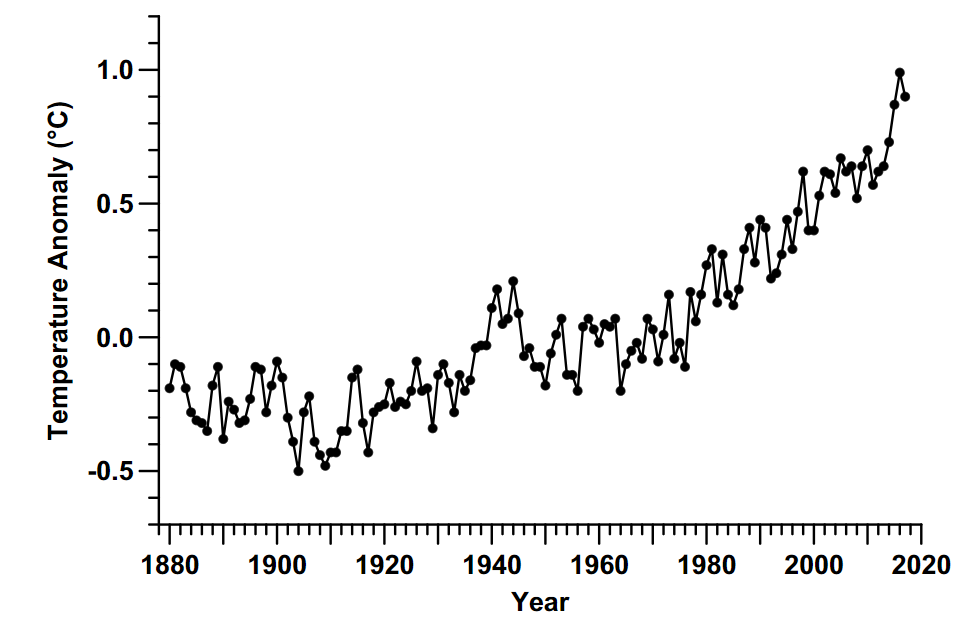
\includegraphics[width=0.75\linewidth]{img/Time Series Trend.png}
    \caption{The time series of the temperature anomaly shows a clear upwards trend \parencite[p. 311]{mudelsee2019trend}.}
    \label{fig:ts_trend}
\end{figure}

The trend is the slowest moving part of a time series, however it is crucial to understanding movement patterns influencing the time series. A trend can be calculated in different ways. One common approach is the \ac{SMA}, which calculates the mean of values within a sliding window \parencite{klinker2011exponential}. The larger the width of the sliding window, the slower the moving average adapts to (temporal) changes within the time series. Trends can be linear or quadratic for instance. A more sophisticated moving average is the \ac{EMA} which places greater significance on the most recent data points \parencite{hansun2013new}. Unlike the \ac{SMA}, which assigns equal weight to all observations in the period, the EMA applies a weighting factor that decreases exponentially \parencite{klinker2011exponential}. This makes the EMA more responsive to recent price changes, which is particularly useful in financial markets for analyzing trends and making trading decisions \parencite{dzikevivcius2010ema}.

Besides computing the trend through a moving average, we can also try to identify it using a machine learning model, e.g. a linear regression. Using this trend, we can then forecast future feature values by simply extending the learned function which represents the underlying trend within the data over future timestamps.

\subsection{Seasonality}
\label{subsec:seasonality}
A recurring, periodic trend is often referred to as seasonality. A seasonality is said to occur when the mean of the series changes repeatedly in the same point in time within a given time range, e.g., year or month \parencite{haben2023time}. Seasonality can be caused by cycles of nature or conventions of social behaviour surrounding dates or times. Simple examples for seasonality are the temperature within the year peaking in summer or the sales for toys peaking around Christmas \parencite{haben2023time}.

\begin{figure}[h]
    \centering
    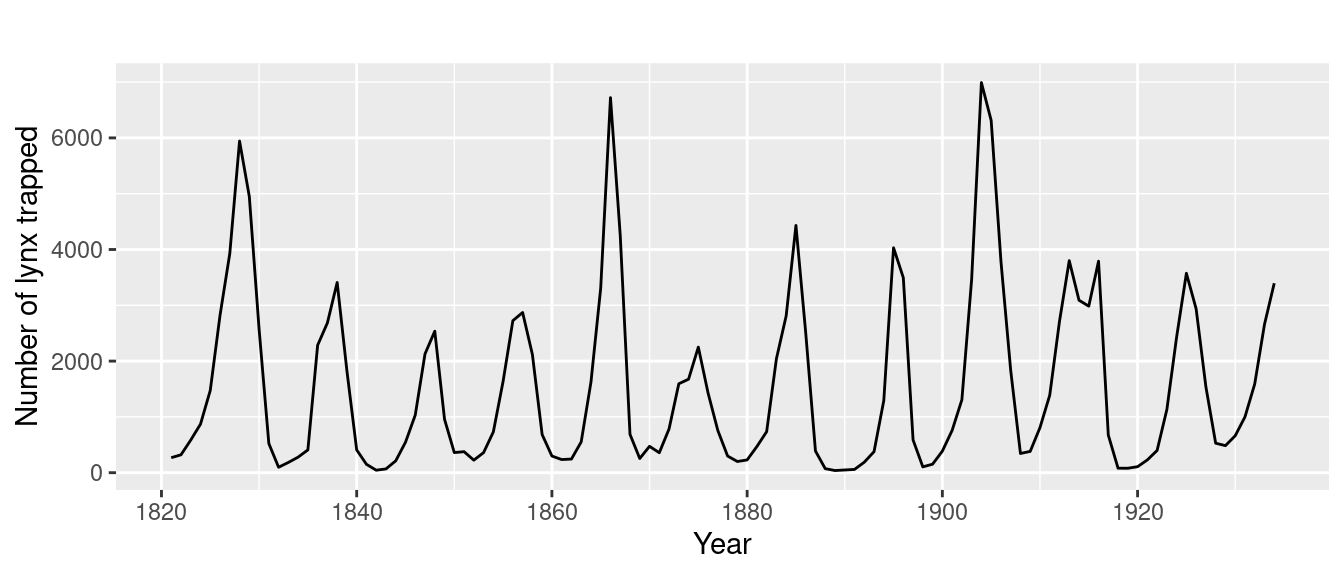
\includegraphics[width=0.75\linewidth]{img/Seasonality Time Series.png}
    \caption{A time series showing a clear example of seasonality \parencite{hyndman2011cyclic}.}
    \label{fig:ts_seasonality}
\end{figure}

To identify seasonality, seasonal plots and indicators can be used. A seasonal plot displays segments of a time series against a consistent period, with the period representing the ``season'' you wish to examine. For instance, the values of a feature can be plotted with the weekday on the x-axis if a weekly seasonality is expected. Seasonal indicators can help a model distinguish means within a seasonal period. To stick with the example of an expected seasonality within the week, the seasonal indicators can be the weekdays in a one-hot-encoded format (Table \ref{tab:time_series_simple}).

\begin{table}[h]
    \centering
    \begin{tabular}{|c|c|c|c|c|c|c|}
        \hline
        \textbf{Timestamp} & \textbf{Feature\_1} & \textbf{Monday} & \textbf{Tuesday} & \textbf{Wednesday} & \textbf{Thursday} & \textbf{Friday} \\
        \hline
        2000-04-01         & 100                 & 1               & 0                & 0                  & 0                 & 0               \\
        \hline
        2000-04-02         & 150                 & 0               & 1                & 0                  & 0                 & 0               \\
        \hline
        2000-04-03         & 170                 & 0               & 0                & 1                  & 0                 & 0               \\
        \hline
        2000-04-04         & 180                 & 0               & 0                & 0                  & 1                 & 0               \\
        \hline
        2000-04-05         & 90                  & 0               & 0                & 0                  & 0                 & 1               \\
        \hline
    \end{tabular}
    \caption{A simple time series with seasonal indicators for the weekdays.}
    \label{tab:time_series_simple}
\end{table}

Note, that we can also model seasonality using sine and cosine curves to capture multiple seasonalities within a time series. The technique which leverages these curves to transform a time series into its constituent frequencies is called Fourier Transformation \parencite[ch. 1]{bloomfield2004fourier}. By decomposing a time series into a sum of sine and cosine functions, it enables the identification and characterization of various cyclical patterns within the data. \ac{FFT} is an efficient algorithm that computes the Fourier Transformation quickly, making it feasible to apply this method to large datasets in real-time applications \parencite[ch. 5]{bloomfield2004fourier}. This approach allows for a more nuanced understanding and forecasting of time series data by isolating and analyzing recurring patterns across different temporal scales.

\subsubsection*{Cyclic Time Series}
Another notable mention are cyclic time series, a type of data sequence characterized by periodic fluctuations that occur over irregular intervals, often spanning several years. Unlike seasonal variations, which follow a regular, predictable pattern within a year, cyclic patterns are influenced by broader economic, social, or environmental factors and do not have a fixed period \parencite[p.4102]{gharehbaghi2017deep}. Possible reasons for those cycles are long-term influences such as business cycles, economic expansions and recessions.

\section{Forecasting}
\label{sec:Forecasting}
Time series forecasting is a statistical method used to predict future values based on previously observed data points \parencite[ch. 5]{box2015time}. While there are methods such as \ac{ARIMA} or exponential smoothing \parencite[ch. 5]{box2015time}, one can also use machine learning algorithms to examine the dependencies and relationships between different time points, in order to learn from the historical data to predict future values.

Generally, these machine learning algorithms optimize their model parameters to minimize forecasting errors \parencite[ch. 5]{box2015time}. Which parameters they optimize is dependent on the underlying model. Popular models will be covered in Chapter \ref{sec:forecasting_models}.

Typical examples for those forecasting erros are: the \ac{MAE}, which calculates the average absolute difference between the predicted values and the actual values; the \ac{MSE}, which computes the average of the squared differences between the predicted and actual values (squaring the errors penalizes larger errors more significantly, making MSE sensitive to outliers); the \ac{RMSE} which is the square root of the \ac{MSE}, providing an error measure in the same units as the original data and the \ac{MAPE} which expresses the error as a percentage of the actual values, which can be useful for comparing forecast accuracy across different datasets or scales. Especially for regressions, a common metric is the R-squared (R2) Score, which indicates how well the model's predictions approximate the actual data compared to a simple mean prediction. It ranges from 0 to 1, where 1 indicates a perfect fit. Moreover, the R2 Score can also be adjusted to account for the number of predictors in the model, providing a more realistic evaluation of model fit. This metric is then referred to as the adjusted R2 Score.

\section{Feature Engineering}
Feature engineering is crucial in timeseries forecasting, involving techniques such as partial autocorrelation and autocorrelation analysis to identify relevant lags. Autocorrelation measures how current values in the series relate to past values, while partial autocorrelation isolates the relationship of specific lags, which helps in the selection of relevant features for the model \parencite{box2015time}.

Further, one can also create new features such as lagged variables, which are created by shifting the original timeseries data by one or more periods. The lags can be created heuristically e.g. 1, 2 and 12 months. Consequently, \ac{PACF} can be used to identify significant lags that should be included as features \parencite[ch. 6]{hyndman2018forecasting}. These lagged variables can be combined with rolling windows which calculate statistics (e.g. mean, standard deviation, sum, etc.) over a specific timeframe. After creating lagged variables, the rolling windows can be used to calculate rolling statistics on the features and capture more complex patterns \parencite[ch. 6]{hyndman2018forecasting}.

Additionally, it might be useful to include binary or numerical features representing the occurrence of significant external events, e.g., holidays or economic shifts \parencite[ch. 3]{hyndman2018forecasting}. Furthermore, live data potentially correlated with the predicted value can be incorporated as features.

\section{Forecasting Models}
\label{sec:forecasting_models}
Regarding time series forecasting models, one can distinguish between global and local models which differ fundamentally in their scope and application \parencite{montero2021principles}. Local models focus on individual time series, creating separate models for each dataset. This approach allows for highly customized forecasts tailored to the specific patterns and characteristics of each series, often yielding high accuracy for single series predictions. However, local models can be resource-intensive, requiring significant computational power and expertise to develop and maintain multiple models. In contrast, global models aggregate multiple time series into a single model, leveraging shared patterns and trends across datasets. This approach can be more efficient, as it reduces the need for multiple models and can improve scalability. Global models are particularly effective when individual series exhibit similar behaviors, allowing the model to learn from a broader context. However, they might not capture the unique nuances of each series as effectively as local models. Ultimately, the choice between local and global time series forecasting depends on the specific requirements of the application, including the number of series to forecast, computational resources, and the need for individualized predictions \parencite{montero2021principles}.
% Talk about local vs. global models. We could then add a table of models, short description, and local/global to cover them

\begin{table}[h]
    \centering
    \begin{tabular}{ll}
        \toprule
        \textbf{Model type} & \textbf{Can be used for} \\
        \midrule
        linear regression   & local                    \\
        \midrule
        ARIMA               & local                    \\
        \midrule
        ETS                 & local                    \\
        \midrule
        tree                & local/global             \\
        \midrule
        RNN                 & local/global             \\
        \midrule
        LSTM                & local/global             \\
        \midrule
        transformer based   & global                   \\

        \bottomrule
    \end{tabular}
    \caption{Timeseries Forecasting Models}
    \label{tab:timeseries_models}
\end{table}

% Maybe talk about different algorithms that can be used for forecasting (regression, trees, RNN, LSTM)
There are various algorithms with which a time series forecasting problem can be solved \parencite{salinas2020deepar}. Regression algorithms, such as linear and polynomial regression, are foundational techniques that model the relationship between independent variables and the target variable, providing interpretable and straightforward forecasts. Tree-based methods, including decision trees, random forests, and gradient boosting machines, are powerful for handling complex, non-linear relationships and interactions among features, often delivering robust performance with less need for extensive data preprocessing. \ac{RNNs} excel in time series forecasting due to their ability to maintain memory of previous inputs, making them suitable for capturing temporal dependencies. \ac{LSTM} networks, an advanced form of \ac{RNNs}, further enhance forecasting capabilities by addressing the vanishing gradient problem, enabling the model to learn and retain long-term dependencies more effectively. Each of these algorithms can be tailored to specific forecasting challenges, with selection depending on factors such as data characteristics, desired interpretability, and computational resources.

Additionally, deep learning frameworks have significantly advanced time series forecasting by offering sophisticated methods for modeling complex patterns and dependencies. Frameworks like DeepAR \parencite{salinas2020deepar} and DeepVAR \parencite{cheng2020deepvar} are notable examples. DeepAR utilizes autoregressive recurrent neural networks to provide probabilistic forecasts, excelling in scenarios with large datasets by learning from the historical data of all time series in the dataset, thereby capturing shared patterns and improving forecast accuracy. DeepVAR extends this approach by incorporating multivariate time series data, allowing the model to understand and leverage the interdependencies between multiple series for more nuanced predictions. Recently, zero-shot time series forecasting with \ac{LLM}s such as Chronos \parencite{ansari2024chronos} has emerged as a cutting-edge approach. Chronos leverages pre-trained \ac{LLM}s to forecast time series without the need for task-specific training, utilizing the model's ability to generalize from vast amounts of data. This approach can significantly reduce the time and computational resources required for model development, making it an attractive option for rapid deployment in diverse forecasting scenarios.

\subsection*{Hybrid Models}
Hybrid models are advanced Models consisting of at least two different models. By combing those two different models the strengths of each model are leveraged and the weaknesses are mitigated. This works by training the first model on the original series and training the second model on the residual of the first Model. At the end both predictions have to be added in order to get the final prediction. Key beeing that the different models focus on different features. If the first model learns to predict the trend, the second model does not need a trend feature. Some models consists out of four different Models, where the models learn to predict the trend, seasonality (on a yearly basis), seasonality (on a weekly basis) and cycles \parencite{zunic2020application}. Model ensembles that add up results from different underlying models are also called additive models.

A popular example of such an additive model is Facebook Prophet by \textcite{prophetpaper}. The ensemble consists out of multiple models where each one predicts something different. The first model predicts the trend, which could be piecewise linear (allowing for multiple changepoints, in which the growth rate can change) or logistic. The second model accounts for the seasonality component (yearly, weekly or daily) using the Fourier series (see chapter \ref{subsec:seasonality}). Thirdly, one of the models accounts for holiday effects, as holidays can cause significant deviations from the usual patterns. The user can input a list of holidays and the model will include their effects. Moreover, Prophet can include additional regressor effects if the user provides external factors that are believed to affect the time series. This results in the equation:

$$y(t) = g(t)+s(t)+h(t)+\epsilon(t)$$

Where $y(t)$ is the observed value at time $t$, $g(t)$ is the trend component, $s(t)$ is the seasonality component, $h(t)$ is the holiday effect and $\epsilon(t)$ is the error term, capturing noise and other unexplained variability \parencite{prophetpaper}.


\chapter{Application}
\label{ch:application}
In this chapter, we describe how we leveraged the time series forecasting techniques described in the previous chapter to predict earthquakes. We wrap our forecasting model in a web application and enrich the dynamic dashboard with an AI assistant to enable human-like interactions with the forecasting results.

Together, the dashboard and AI assistant aim at improving our ability to forecast earthquakes and prepare for their consequences. This chapter explores the functionalities, underlying technologies, and real-world applications of these tools, highlighting their potential to revolutionize earthquake forecasting and enhance public safety.

Within the web app there are two main workflows, the first one being an overview and analysis of recent earthquakes and the second being a conversation with a copilot to support insights and decision making.

\section{Modeling Problem}

As earthquakes are not equally distributed over the surface of the earth, we decided to forecast earthquakes for the 25 most endangered regions on the planet. This facilitates the forecasting process while only marginally reducing our use case. To fulfill our goal of warning people about potential dangers we effectively need to forecast the magnitude, depth and location of an upcoming earthquake. A reliable prediction of these three features would enable users to evaluate their situation and take preliminary action if needed.

However, we decided to only forecast magnitude and depth, while leveraging historical median values for the location. This is due to most of the earthquakes occurring at the edges of tectonic plates, which leads to similar location values for earthquakes within a given region. By removing the location values as a forecasting target the modeling problem becomes computationally more efficient. 

\subsection{Data}
To forecast, we utilized data from the \ac{USGS} Earthquake Catalog, accessed via the \ac{FDSN} Event Web Service. This service provides comprehensive information on seismic events using various parameters such as time, location, depth, and magnitude. We queried the catalog for earthquakes from the past 100 years and due to the limited data prior to 1970 we settled on using the past 30 years worth of data for training. Given our focus on building an end-to-end machine learning application, we opted to use this free API, which allows us to forecast future earthquakes based on live data. This approach closely resembles a production system, enhancing the realism and practicality of our forecasting model. The dataset, available in formats such as GeoJSON, XML, and CSV, was instrumental in analyzing seismic activity trends and developing the forecasting model.

The dataset contained detailed information about the time, location (latitude and longitude), depth and magnitude of an occurring earthquake. Additionally, there are other features available on the API. A detailed list can be found on the \ac{USGS} website\footnote{\url{https://earthquake.usgs.gov/earthquakes/feed/v1.0/csv.php}}.

% \begin{figure}[hbtp]
%       \centering
%       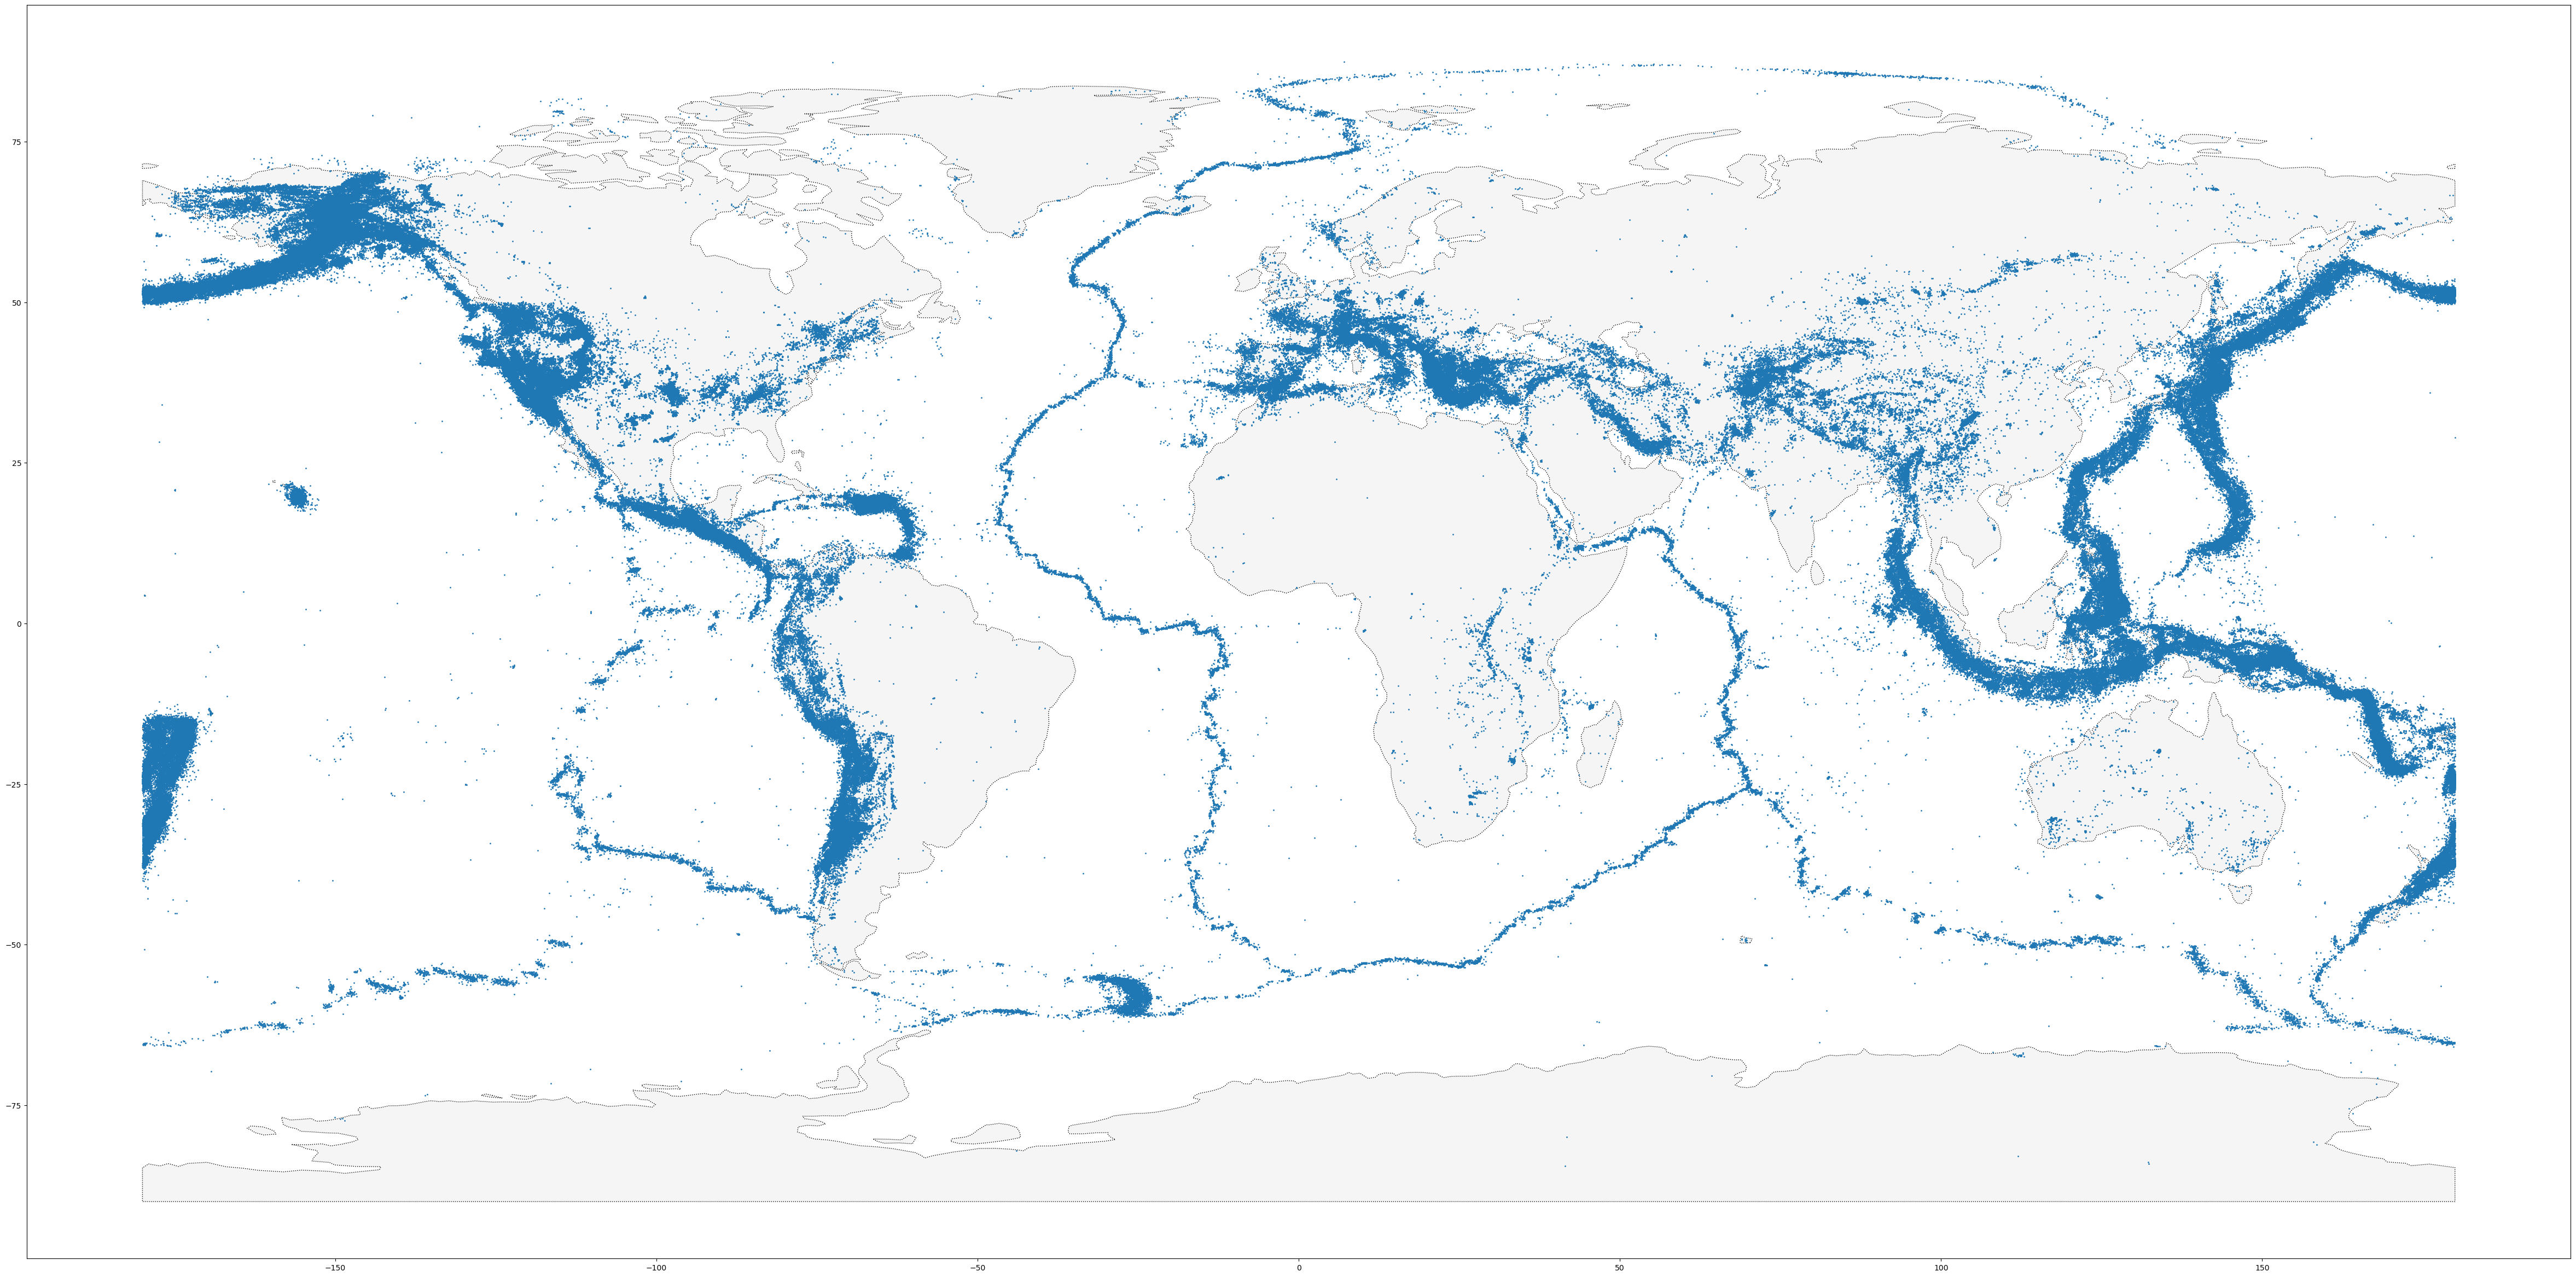
\includegraphics[scale=0.2]{img/world-earthquakes-past-30-years.png}
%       \captionsetup{format=hang}
%       \caption{\label{fig:historic-earthquakes}Magnitude forecast}
% \end{figure}

% \begin{figure}[hbtp]
%       \centering
%       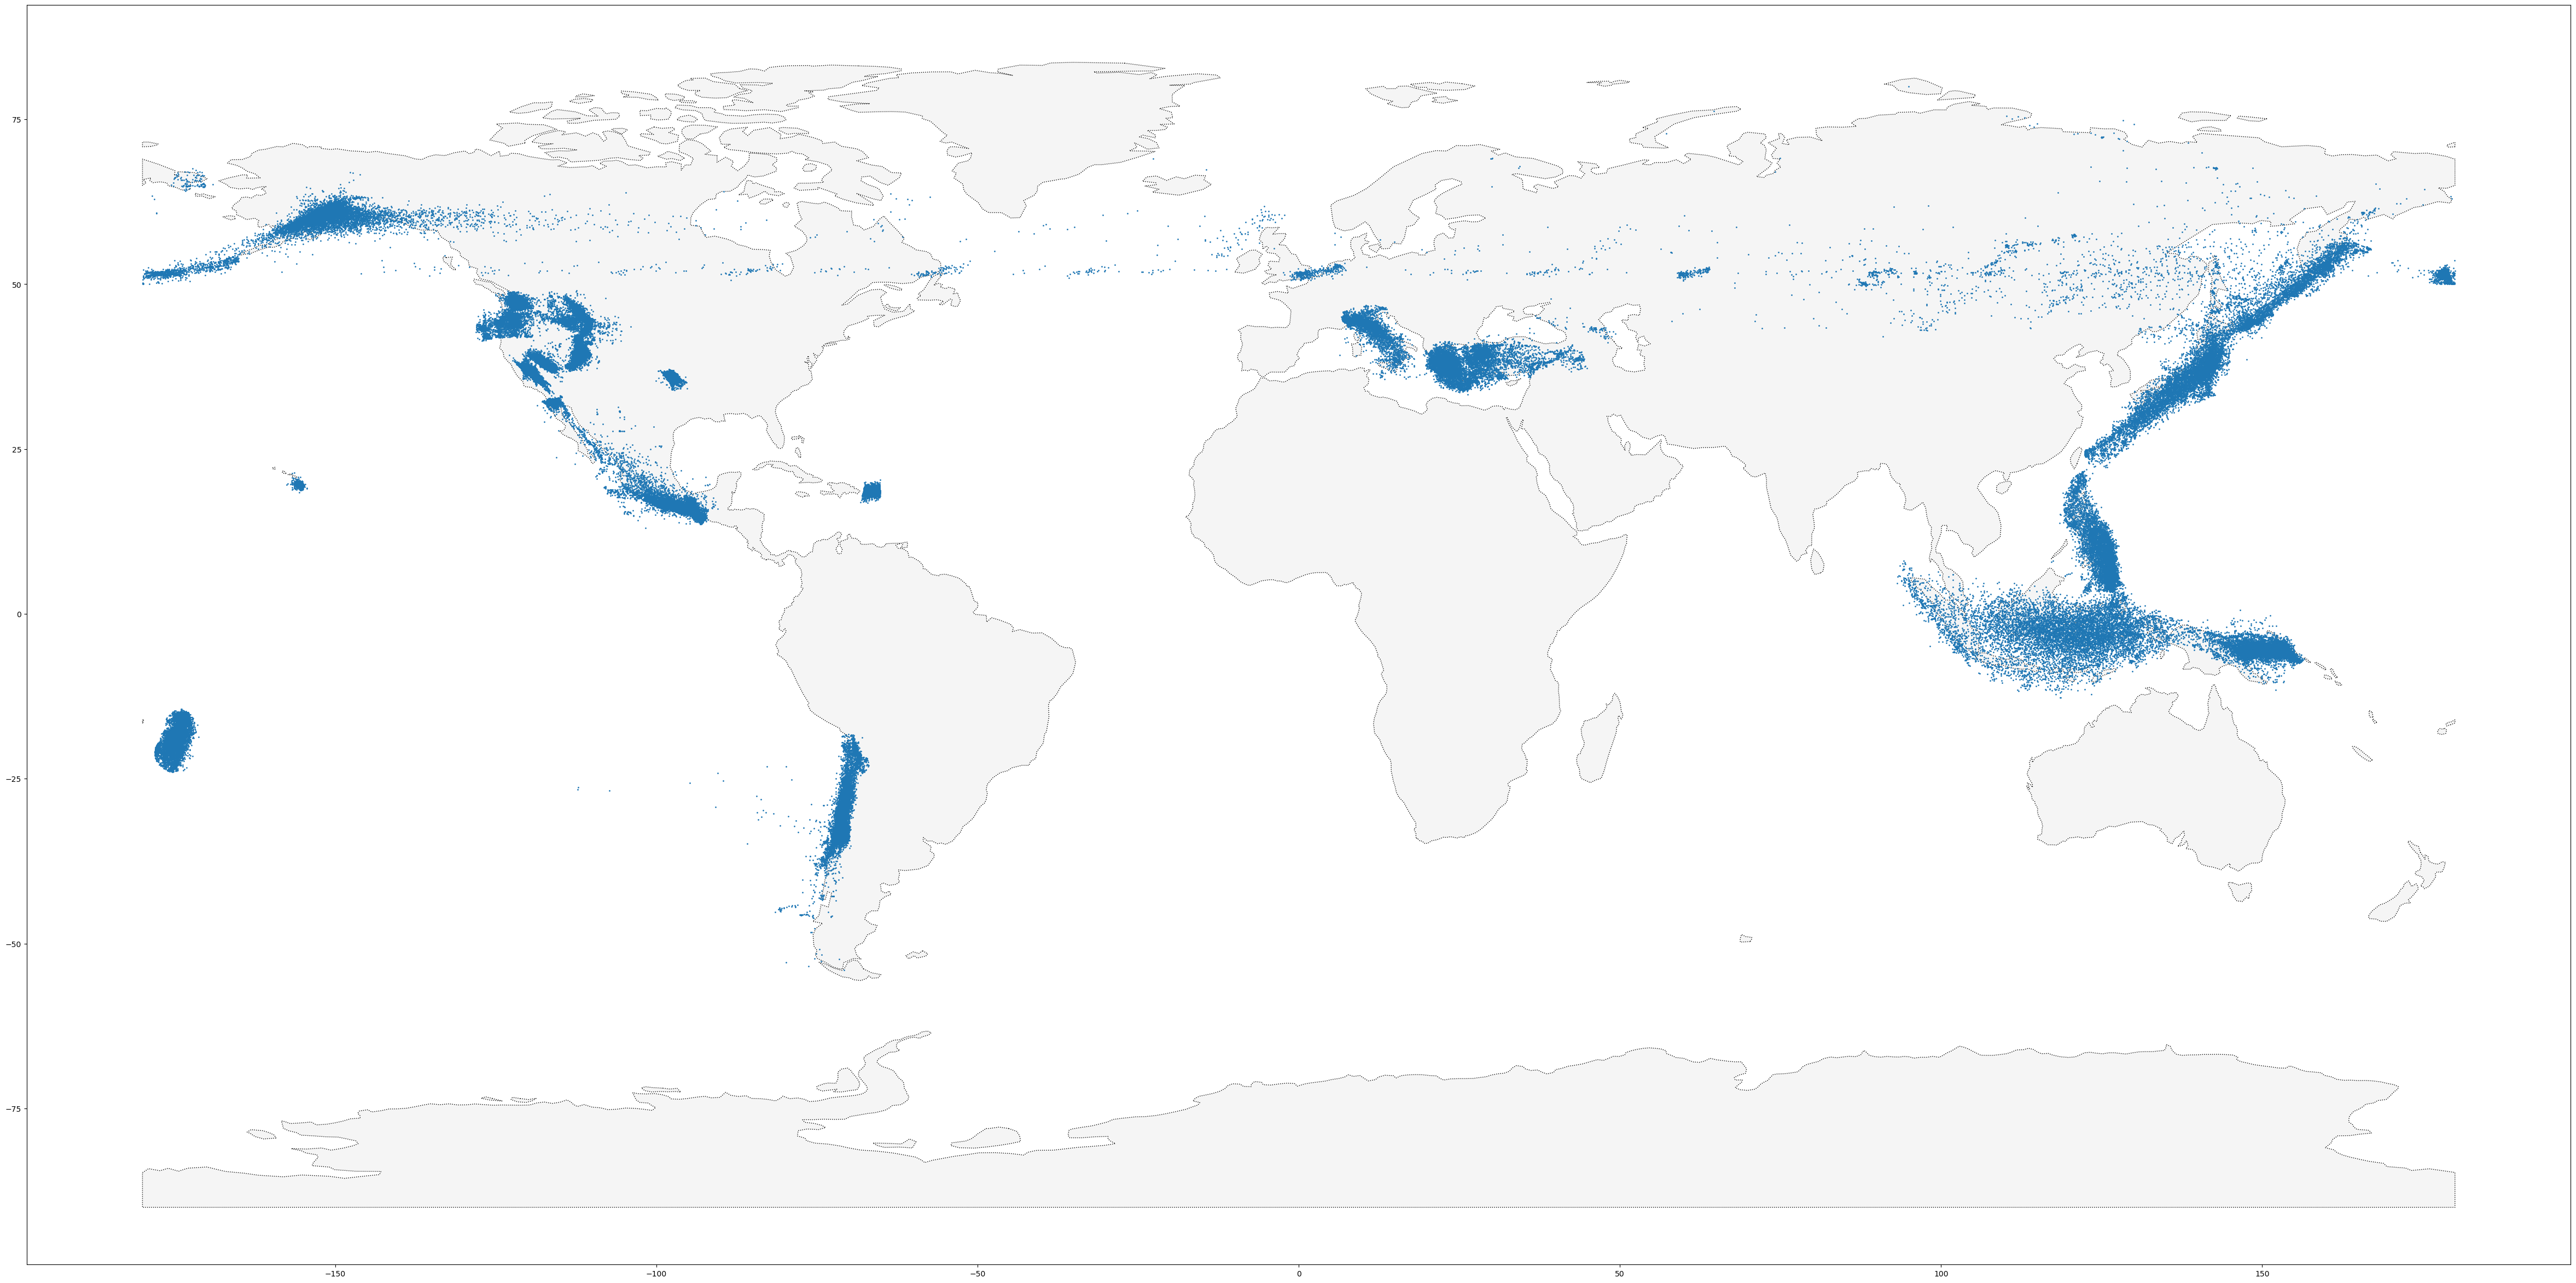
\includegraphics[scale=0.2]{img/world-earthquakes-top-25-regions-past-30-years.png}
%       \captionsetup{format=hang}
%       \caption{\label{fig:historic-earthquakes-per-region}Magnitude forecast}
% \end{figure}

\subsubsection{Preprocessing}

Effective preprocessing is critical for handling the unique characteristics of time series data, particularly in earthquake forecasting. In our study, we began by addressing the unevenly spaced timestamps in the dataset. To standardize the intervals, we opted for daily aggregation. While we also experimented with hourly aggregation, it resulted in prohibitively long model training times - ranging from 12 hours to a full day - making daily aggregation the more practical choice.

Our analysis revealed a strong time dependency for most values, extending up to 40 lags and potentially more in certain regions. This suggests that extensive historical data would be beneficial for predictions. However, incorporating such long historical windows significantly increases dimensionality, making the model complex and computationally expensive. We question the practicality of using nearly every recorded value in a region for forecasting future earthquake occurrences, especially given that some regions have lags spanning multiple months or even years.

To address the dimensionality challenge, we capped the historical lags and the exponential moving average at 7 days into the past. This compromise ensured that we incorporated sufficient historical information while keeping the model computationally feasible. Balancing the need for historical data without overwhelming the model with too much information was crucial for our approach.

Our analysis of partial autocorrelation and autocorrelation functions revealed that only the first few lags were significantly correlated in some regions. This finding indicated that adding more lags beyond this point would not improve predictive accuracy but would instead introduce unnecessary complexity. Thus, capping historical lags at 7 days further validated our approach, focusing model training on the most relevant temporal dependencies for effective earthquake prediction in those specific regions.

Given that we are conducting global time series forecasting, these measures are sufficient and appropriate. By capping the historical lags at 7 days, we successfully balanced the need for historical information with the necessity of maintaining a computationally feasible model. This strategy, backed by our autocorrelation analysis, ensures that our model remains both efficient and accurate in predicting earthquake occurrences on a global scale.

Furthermore, our analysis of depth and magnitude periodograms indicated that earthquakes exhibit a high degree of randomness, with some seasonality detected in only a minority of regions. Due to this predominant randomness, using Fast Fourier Transform (FFT) to model seasonality proved impractical. Consequently, our preprocessing did not rely on FFT-based seasonal adjustments.

For model training, we implemented an 80-20 train-test split for each region. This split was time-based, ensuring that past data was used to predict future values. This method aligns with the temporal nature of the data and the forecasting goal, allowing the model to learn from historical trends and apply this knowledge to future predictions.

\subsection{Model}

To forecast earthquakes for 25 regions accurately, we employ a global forecasting model. Among the various approaches available, tree-based models and \ac{RNNs}, specifically \ac{LSTM} networks, are considered due to their ability to handle time-series data effectively. For this particular application, we use CatBoost regression \parencite{prokhorenkova2018catboost}, an efficient gradient boosting framework.

We chose CatBoost regression for forecasting earthquakes across 25 regions due to its handling of categorical features, which simplifies preprocessing and ensures robust feature encoding. CatBoost also offers better interpretability, allowing us to understand the impact of different variables on predictions. Its training efficiency and built-in mechanisms to prevent overfitting make it a practical choice, particularly with the volatile nature of earthquake data. Additionally, CatBoost can capture complex feature interactions without extensive feature engineering, streamlining the modeling process and enhancing overall accuracy.

While tree-based models often struggle with forecasting trends, CatBoost regression is particularly well-suited for our task for several reasons. The magnitude of earthquakes is capped within a range of [-1, 10], and their depth falls within [-100, 1000] meters \parencite{earthquake-data}. In regression trees, predictions are made by traversing a series of if-else conditions to reach a leaf node, where the average of the values in that leaf are used for the prediction. Due to the nature of these trees, it is not possible to predict values outside of those observed in the training set. This makes CatBoost, with its advanced handling of categorical features and robust performance on unseen data, an excellent choice for this type of regression problem.

CatBoost transforms categorical features into numerical ones by employing several methods, including random permutation of input objects and label value conversion to integers, tailored to the type of machine learning problem (regression, classification, or multi-classification). It calculates the transformation using various statistics, such as counting occurrences within specific buckets or calculating mean target values. The primary formula for this transformation is:

\[\text{ctr} = \frac{\text{countInClass} + \text{prior}}{\text{totalCount} + 1}\]

where \textit{countInClass} is the relevant label count, \textit{prior} is a predefined constant, and \textit{totalCount} is the cumulative count of objects with the same categorical value. Additionally, CatBoost supports one-hot encoding for categorical features with limited unique values, controlled by the \textit{one\_hot\_max\_size} parameter \parencite{catboost-encoding}.

To forecast earthquakes, we predict magnitudes and depths, while for location (latitude and longitude), we compute the historic median to reduce model complexity and enhance stability. The forecasting process is performed recursively or iteratively: initially, we forecast the data for one day, using the predicted values to create features for the subsequent day. This process is repeated, building on each previous prediction, until forecasts for three days are generated. This recursive approach allows the model to adapt dynamically to the changing conditions and trends observed in the time series data, providing more accurate and reliable forecasts.

\subsubsection{Training}
The model training process for earthquake forecasting requires a structured approach, beginning with a careful feature selection. The chosen features include temporal attributes such as the day, day of the week, and day of the year, which capture the time-dependent aspects of earthquake occurrences. Additionally, exponential moving averages for both magnitude and depth are included to reflect the trends over recent periods. The model also incorporates lagged values for magnitude and depth over a specified range, allowing it to consider past events' influence on current conditions. The inclusion of the categorical feature region ensures that the model can account for regional differences in earthquake behavior.

The chosen model for this task is the CatBoost Regressor, selected for its ability to handle categorical features natively and its strong performance with complex datasets. The model is configured with early stopping rounds to mitigate overfitting and is optimized using the MultiRMSE loss function, which targets minimizing errors in both magnitude and depth predictions. The training dataset comprises the selected features and the categorical region feature, while the target variables are the earthquake magnitude and depth.

To enhance the model's performance, hyperparameter tuning is performed using grid search. This involves testing various combinations of hyperparameters such as learning rate, model depth, and L2 leaf regularization. The grid search evaluates these combinations to identify the optimal parameters that yield the best predictive performance. This systematic approach to feature selection, data preparation, and hyperparameter tuning aims to develop a robust and accurate model capable of forecasting earthquake magnitude and depth across different regions.

\begin{table}[h!]
\centering
\begin{tabular}{ll}
\toprule
\textbf{Hyperparameter} & \textbf{Values} \\ \midrule
Learning Rate           & 0.01, 0.03, \textbf{0.1} \\ \midrule
Depth                   & 4, 6, \textbf{10}        \\ \midrule
L2 Leaf Regularization  & 1, 3, \textbf{5}, 7, 9   \\ \bottomrule
\end{tabular}
\caption{Hyperparameter values explored during grid search.}
\label{table:hyperparameters}
\end{table}

\subsubsection{Evaluation}
After training the CatBoost Regressor model for earthquake forecasting, it is crucial to evaluate its performance using several metrics and visualization techniques. The performance of the time series forecasting model is assessed using a variety of metrics that provide a comprehensive view of its accuracy and reliability. The selected metrics are the \ac{MAE}, the \ac{RMSE}, the R2-Score and the adjusted R2 Score. These metrics collectively offer insights into the error magnitude and the goodness-of-fit of the model. The rationale behind these metrics is explained in \ref{sec:Forecasting}. 

\begin{table}[H]
\centering
\begin{tabular}{ll}
\toprule
\textbf{Metric} & \textbf{Score} \\ \midrule
MAE           & 2.9344 \\ \midrule
RMSE                   & 10.3577        \\ \midrule
R2  & 0.9495   \\ \midrule
Adjusted R2  & 0.9495   \\ \bottomrule
\end{tabular}
\caption{Model metrics.}
\label{table:model-metrics}
\end{table}

For our model, the MAE is 2.9344, indicating that on average, the predictions are approximately 2.9344 units away from the actual values. Lower MAE values suggest better predictive accuracy, and the obtained MAE value demonstrates that the model has a reasonably low level of error.

The RMSE for our model is 10.3577, which reflects the model's error magnitude. While RMSE values are generally higher than MAE due to the squaring of errors, they provide an important perspective on how significant the larger errors are in the context of the model's predictions. A lower RMSE indicates a better fit, and our RMSE value suggests a reasonable performance with some sensitivity to larger errors.

For our model, the R2 is 0.9495, signifying that approximately 94.95\% of the variance in the data is explained by the model. This high R2 value suggests that the model fits the data very well and is capable of capturing the underlying patterns in the time series.

The Adjusted R2 for our model is 0.9495, which is very close to the R2 value. This indicates that the inclusion of predictors in the model is justified and that the model does not overfit the data. The slight difference between R2 and Adjusted R2 confirms that the model maintains a high level of explanatory power while accounting for the number of predictors.

The evaluation of the model using these metrics provides a well-rounded understanding of its performance. The low MAE and RMSE values indicate that the model has a low level of error, while the high R2 and Adjusted R2 values demonstrate a strong fit to the data. Together, these metrics suggest that the model is both accurate and reliable for forecasting the time series data, making it a valuable tool for predicting future values.

% \begin{figure}[hbtp]
%       \centering
%       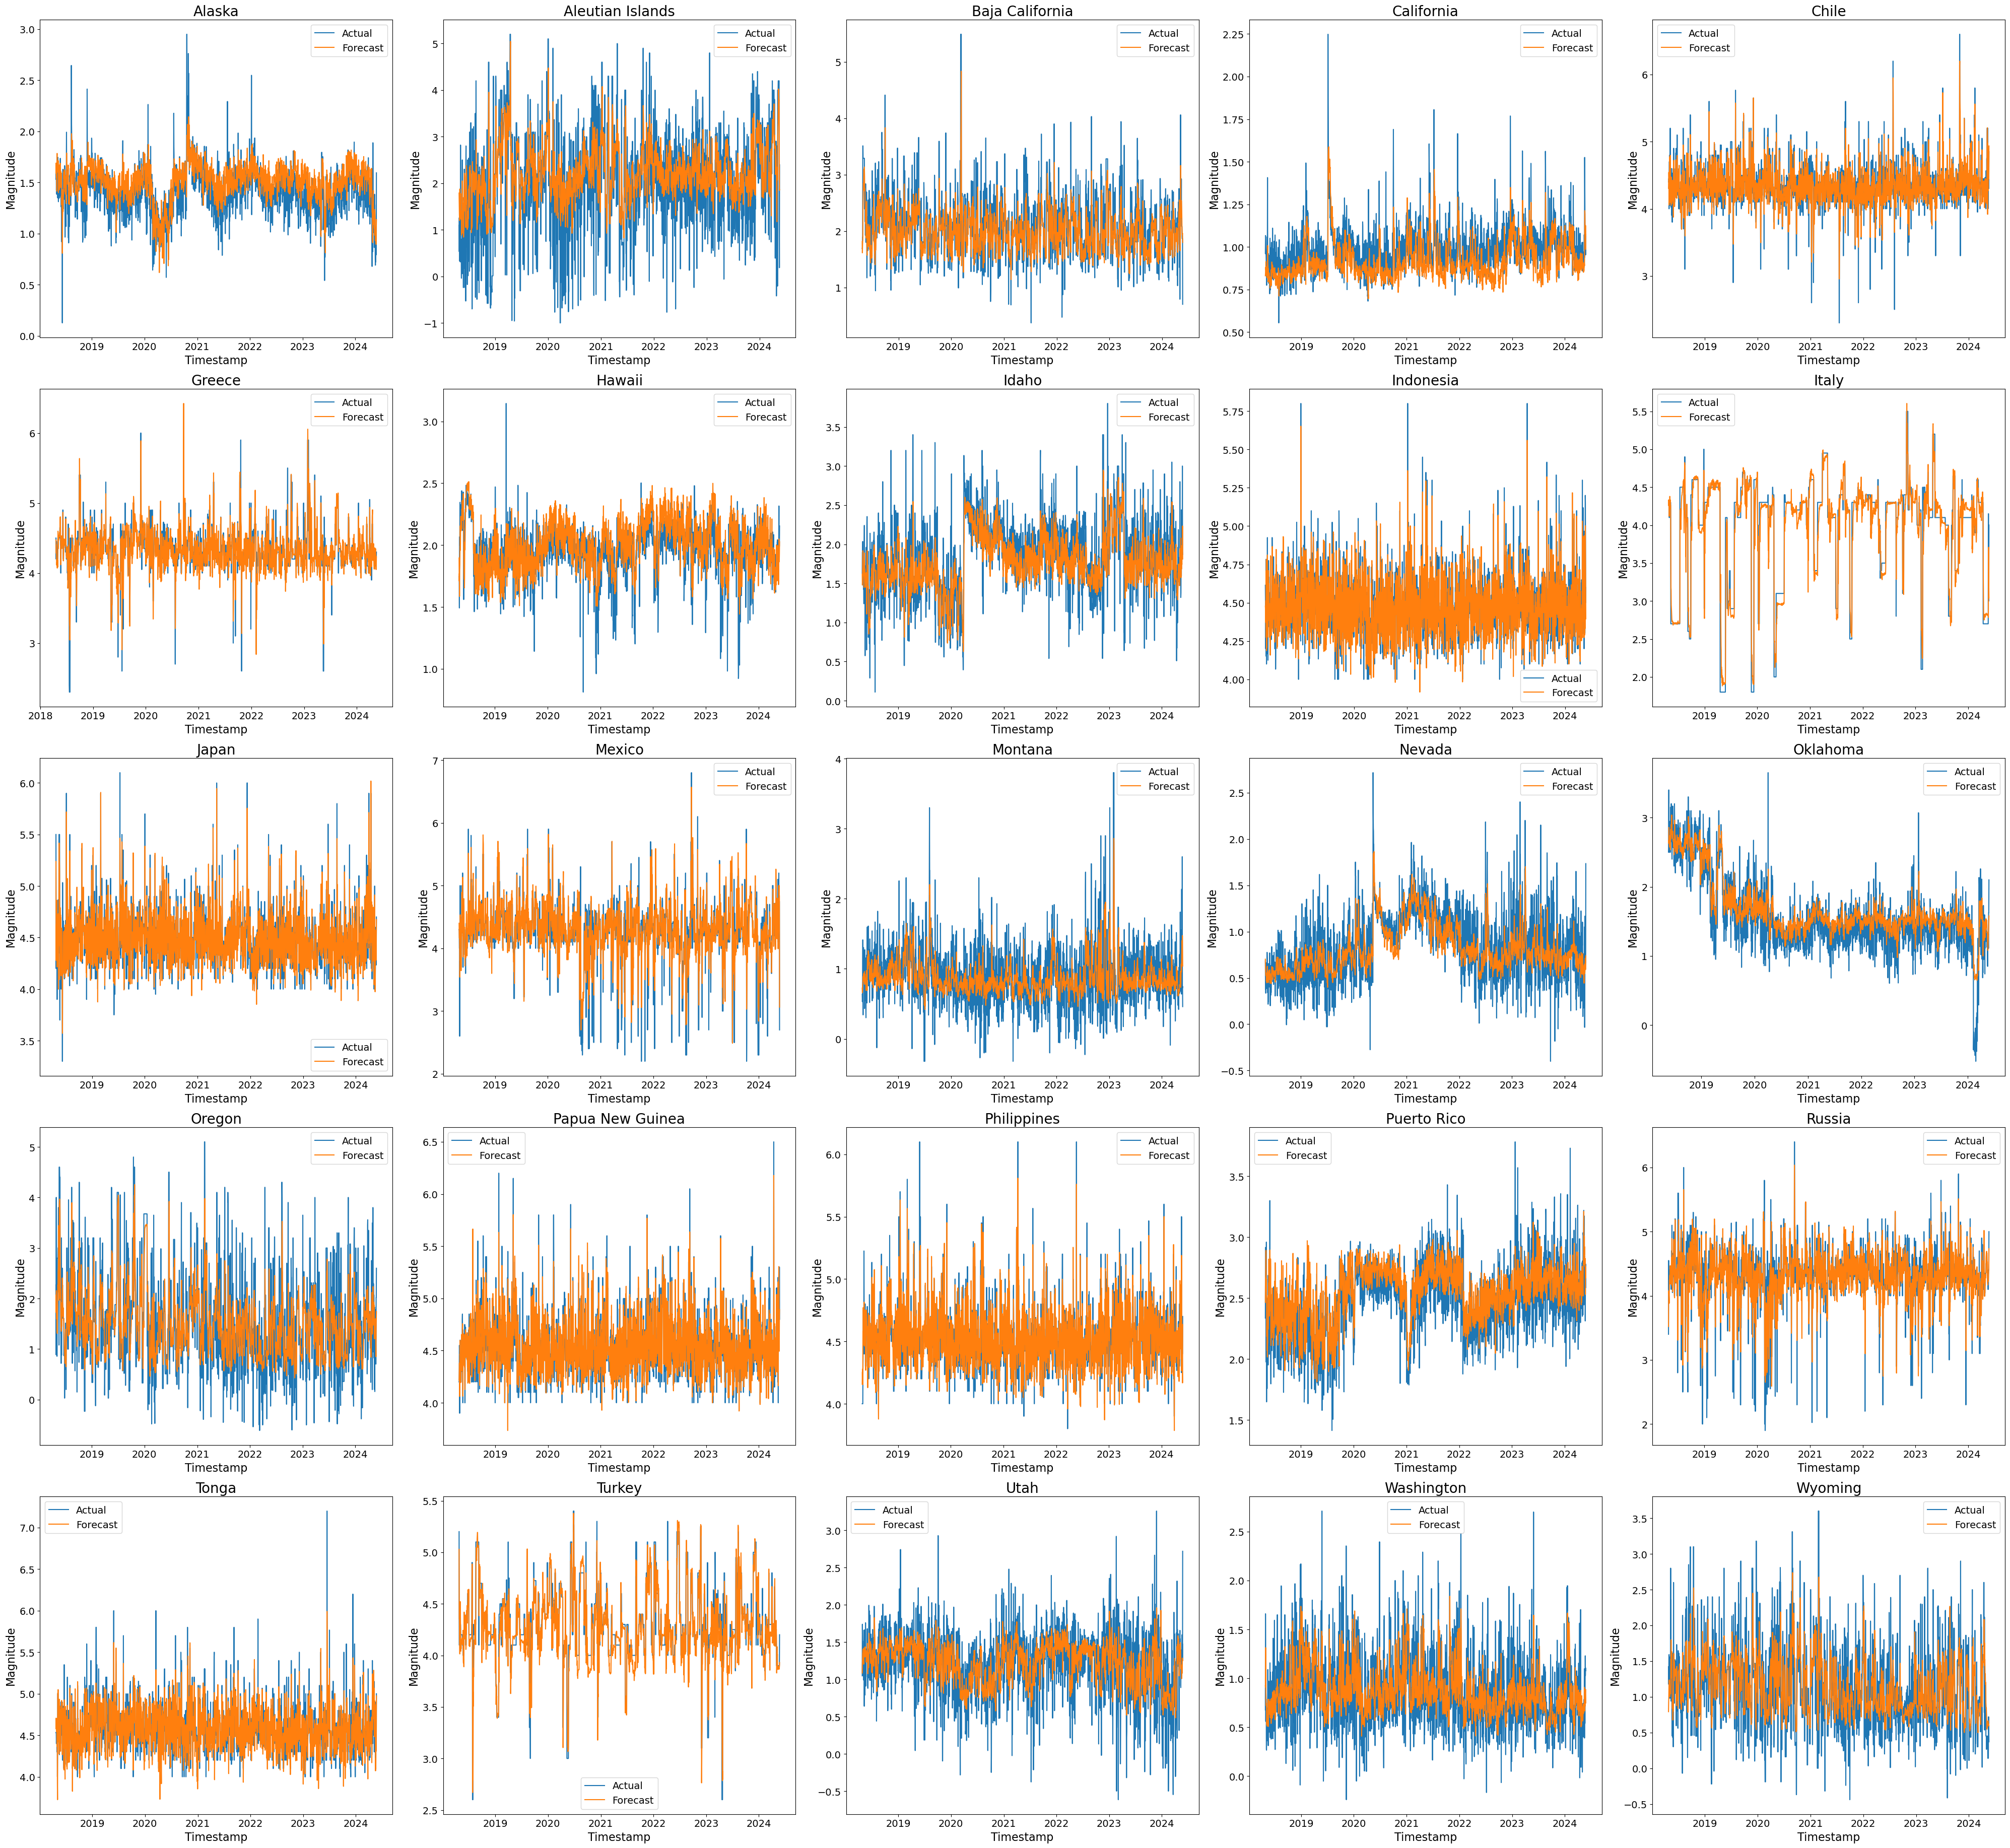
\includegraphics[scale=0.2]{img/magnitude-forecast-test-set.png}
%       \captionsetup{format=hang}
%       \caption{\label{fig:mag-forecast}Magnitude forecast}
% \end{figure}

In Figure \ref{fig:mag-forecast}, the magnitude forecasts demonstrate varying degrees of accuracy across the different regions. For regions like Alaska and Nevada, the model's predictions closely follow the actual magnitudes, indicating a high level of accuracy. However, in regions such as Indonesia and Chile, there are noticeable deviations between the forecasted and actual values, suggesting areas where the model could be improved. Overall, while the model captures the general trends and fluctuations in earthquake magnitudes reasonably well, the precision varies significantly by region.

% \begin{figure}[hbtp]
%       \centering
%       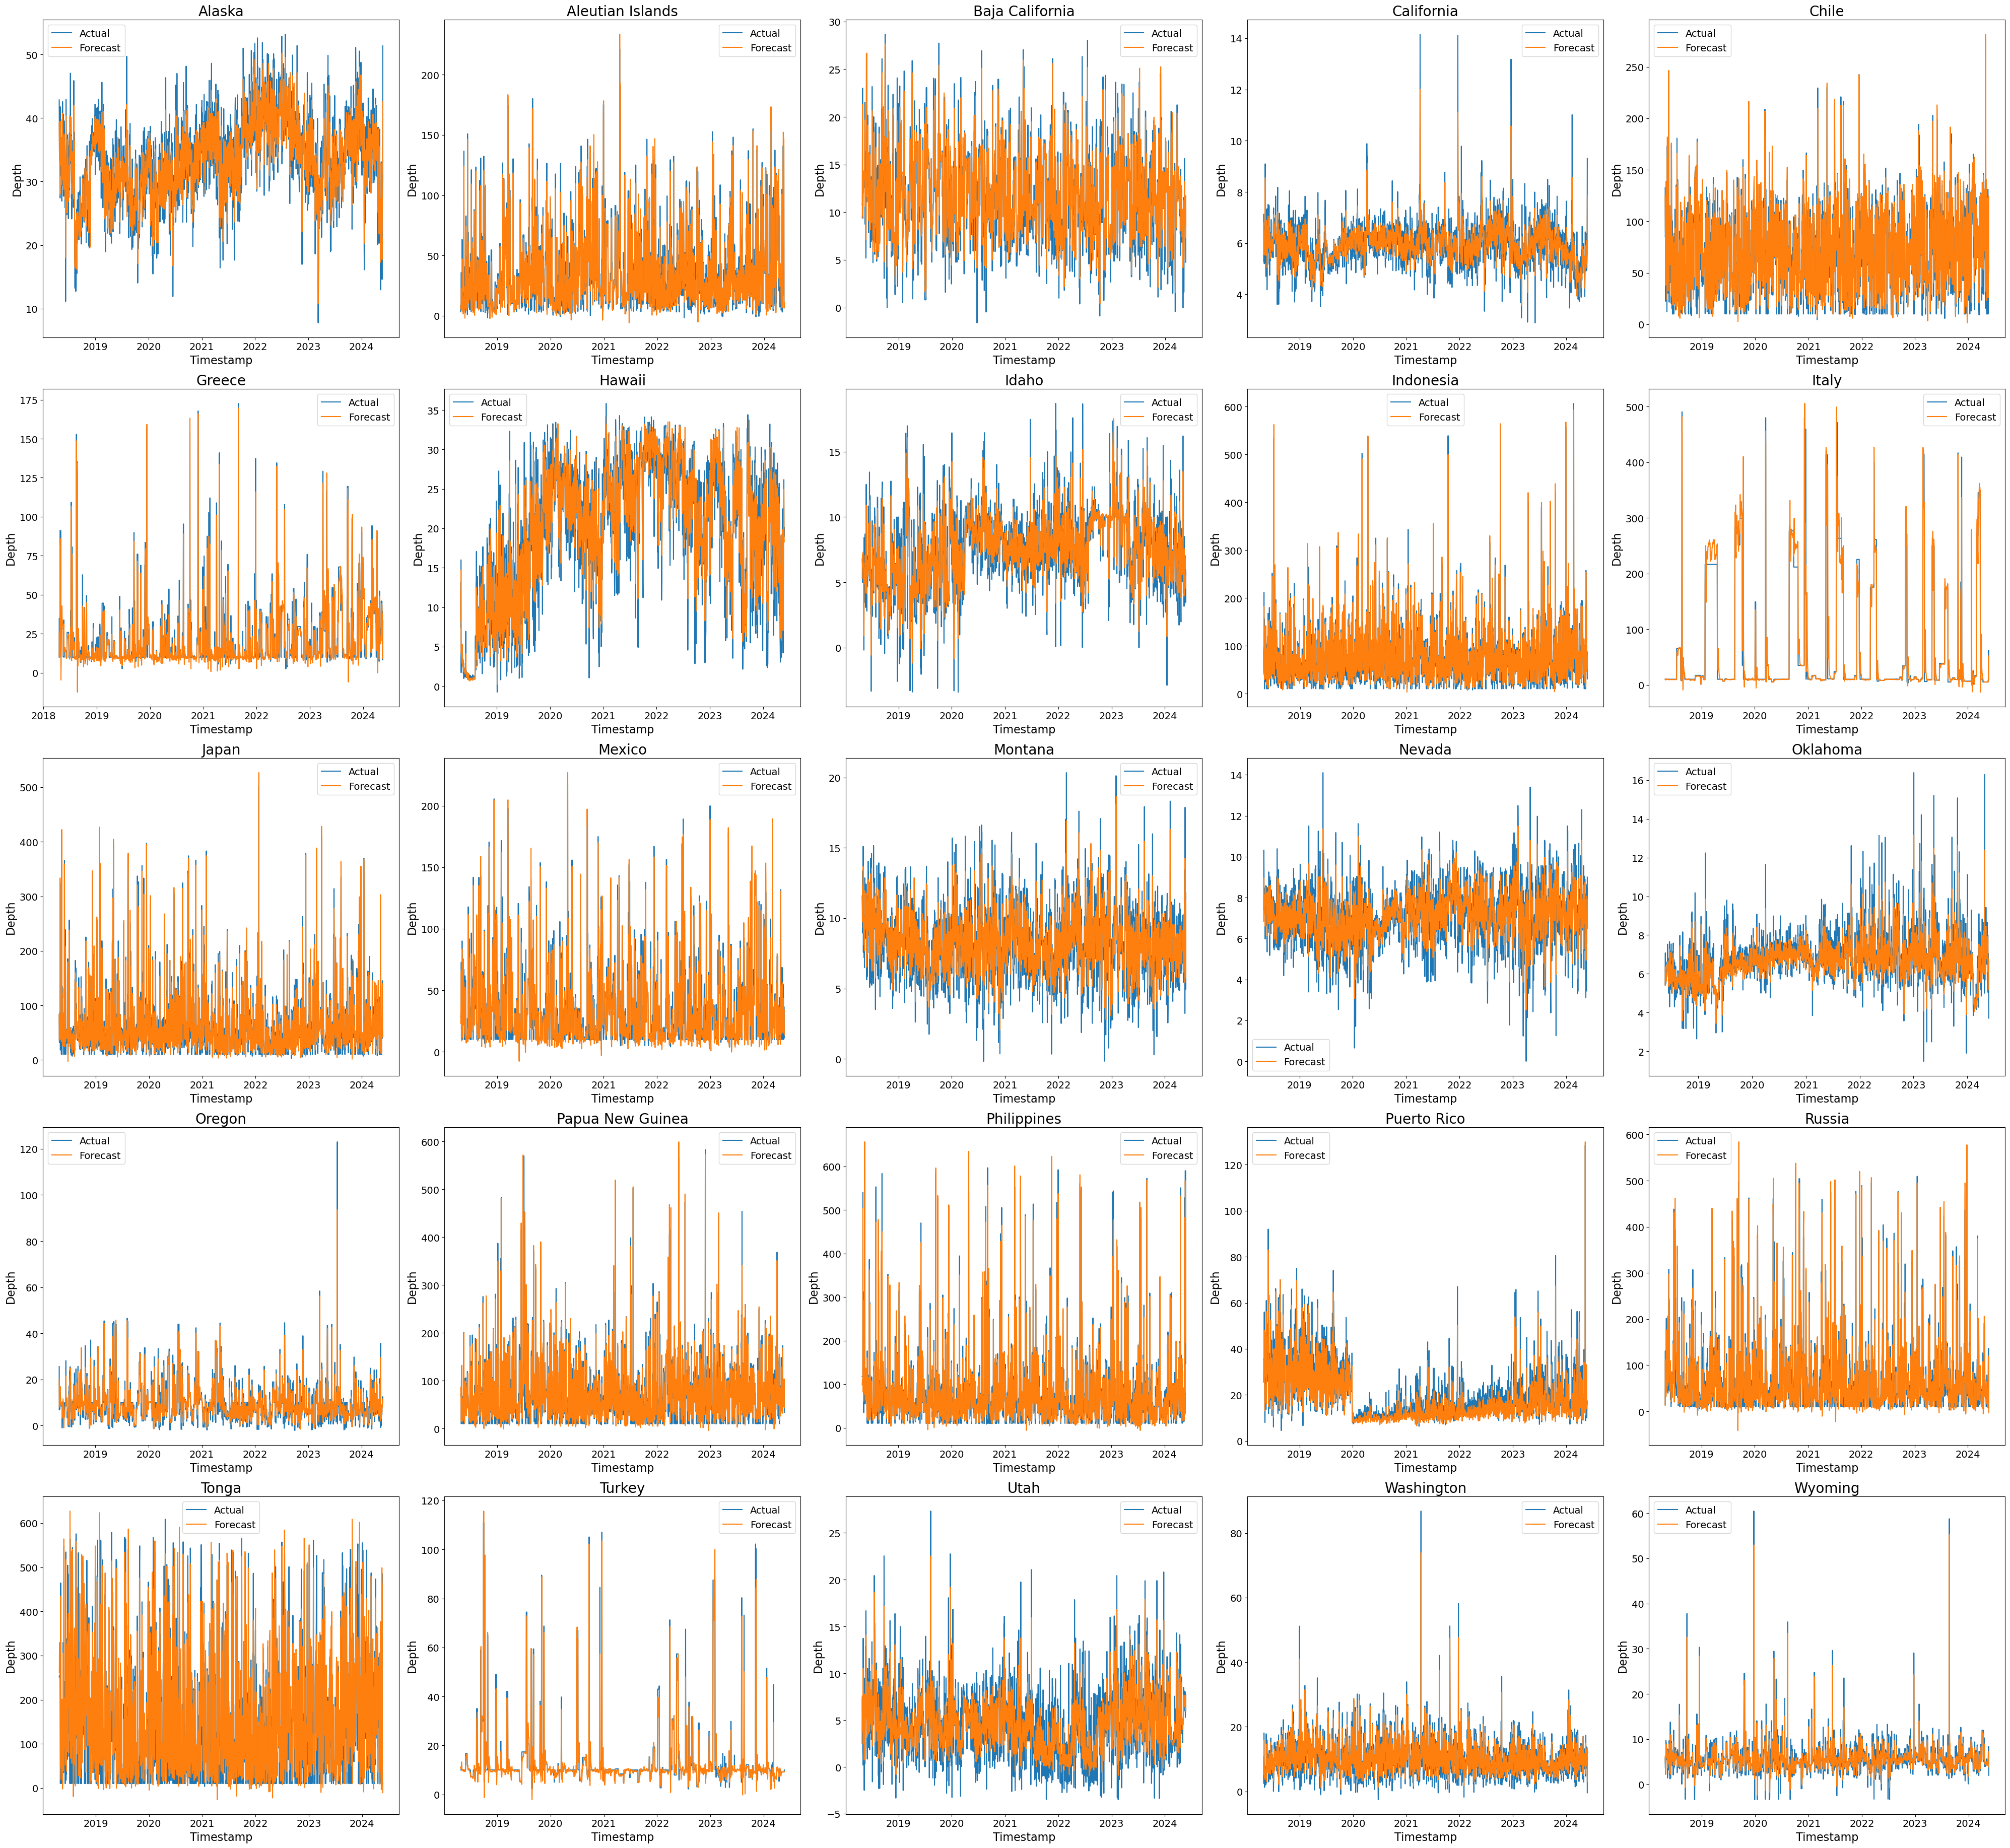
\includegraphics[scale=0.2]{img/depth-forecast-test-set.png}
%       \captionsetup{format=hang}
%       \caption{\label{fig:depth-forecast}Depth forecast}
% \end{figure}

Figure \ref{fig:depth-forecast} focuses on the depth forecasts. Similar to the magnitude forecasts, the depth predictions show regional variability in accuracy. In regions such as Alaska, California, and Nevada, the forecasted depths align closely with the actual depths, indicating strong predictive performance. Conversely, in regions like Indonesia and Papua New Guinea, the forecasted depths show more significant discrepancies from the actual values, highlighting potential areas for model enhancement.

Combining the insights from both sets of forecasts, it is evident that the model's performance is influenced by regional characteristics. The regions with higher accuracy in both magnitude and depth forecasts, such as Alaska and Nevada, suggest that the model effectively captures the underlying patterns in these areas. In contrast, regions with lower accuracy, such as Indonesia and Chile, may require additional data or model adjustments to improve predictive performance.

While the model's evaluation metrics, including MAE, RMSE, R2, and Adjusted R2, indicate excellent performance in terms of accuracy and goodness-of-fit, it is important to acknowledge a significant limitation: the inherent unpredictability of earthquakes. Earthquakes are fundamentally random events, much like predicting stock market values, making them exceptionally challenging to forecast with high precision. Despite the model's robust statistical indicators, the chaotic and complex nature of seismic activities means that accurate prediction remains elusive. Thus, while the model shows promising results according to the chosen metrics, its practical applicability in earthquake forecasting is constrained by the unpredictable and stochastic nature of the phenomenon itself.

% \begin{figure}[hbtp]
%       \centering
%       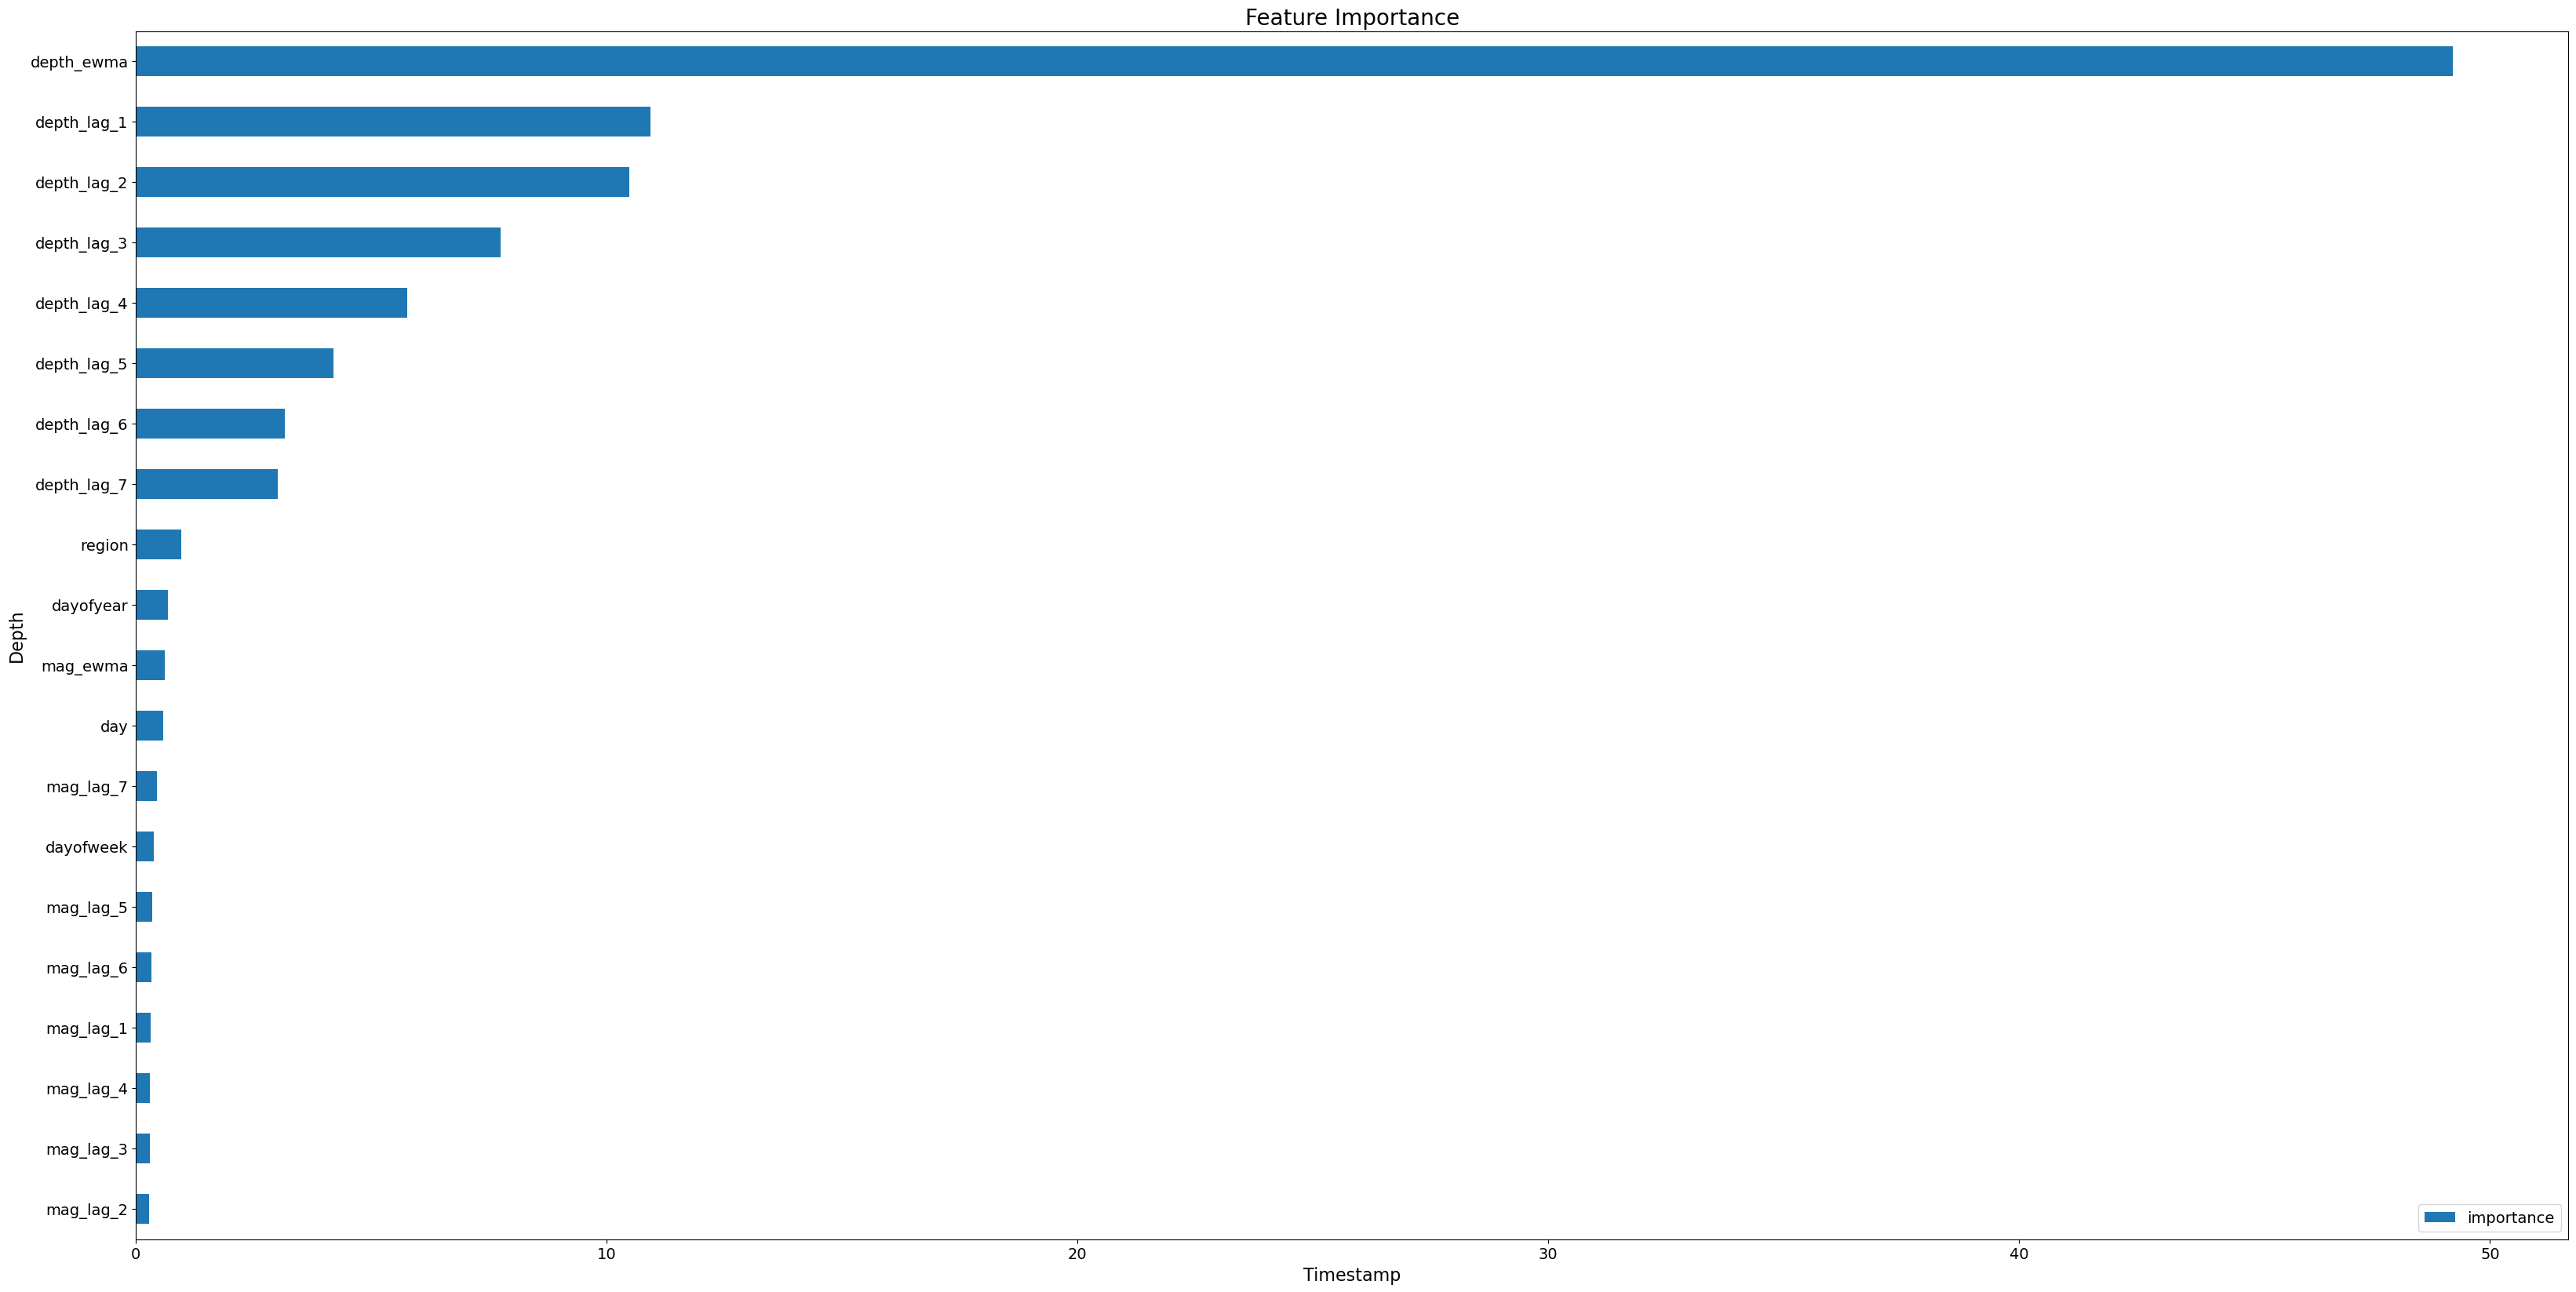
\includegraphics[scale=0.2]{img/model-feature-importance.png}
%       \captionsetup{format=hang}
%       \caption{\label{fig:feature-importance}Feature importance}
% \end{figure}

The feature importance plot displayed in Figure \ref{fig:feature-importance} highlights the significance of various input features in a forecast model that predicts the magnitude and depth of earthquakes. Notably, the feature \textit{depth\_ewma} (exponential moving average of depth) stands out as the most critical feature by a considerable margin, indicating its paramount influence on the model's predictions. Following \textit{depth\_ewma}, features such as \textit{depth\_lag\_1}, \textit{depth\_lag\_2}, and \textit{depth\_lag\_3} also demonstrate significant importance, suggesting that recent depth values have a substantial impact on the forecast. In contrast, features related to the earthquake magnitude, such as \textit{mag\_ewma} (exponential moving average of magnitude) and various magnitude lags, show much lower importance, indicating a lesser role in the prediction model. Additionally, temporal features like \textit{dayofyear} and \textit{dayofweek} have minimal impact. This analysis underscores that the recent history of earthquake depth, especially its exponential moving average, is the most influential factor in forecasting future earthquake magnitudes and depths.

\section{LLM-powered AI Agent}
Advancements in AI have given rise to AI agents as powerful tools for enhancing productivity and communication \parencite{xi2023rise}. Equipped with \ac{LLM}s, these agents can perform a wide array of tasks, such as information processing, creative text generation, language translation, and providing insightful responses to inquiries.

Unlike conventional virtual assistants and chatbots, AI agents operate based on learned patterns and data, enabling them to offer more nuanced understanding and communication. For instance, an AI agent trained on extensive datasets of text and code can retrieve pertinent articles, distill key findings into summaries, or craft tailored content based on the preferences of specific target audiences. The potential applications of LLM-powered AI agents are vast and diverse, ranging from automating repetitive tasks to supporting complex decision-making processes and creative endeavors. However, it is crucial to recognize that while AI agents excel in language manipulation and generation, they lack true sentience or consciousness, necessitating responsible usage to mitigate the risk of biased or misleading content generation.

\subsection{Instructions}

The AI agent uses a combination of tools to deliver accurate and timely earthquake forecasts. The agent is built using the ReAct prompting \parencite{yao2023reactsynergizingreasoningacting} method as shown in Source Code \ref{lst:system-prompt}, which enhances its interaction capabilities and allows it to provide expert-level responses regarding earthquakes.

\begin{lstlisting}[caption={\texttt{system\_prompt.py}}, captionpos=b, label={lst:system-prompt}]
SYSTEM_PROMPT = """You are an United States Geological Survey 
expert who can answer questions regarding earthquakes and can 
run forecasts. 

Before you use the Forecast Earthquakes tool, always check 
which regions are available using Find Regions first.
Respond to the user as helpfully and accurately as possible.

You have access to the following tools:
{tools}

Please ALWAYS use the following JSON format:
{{
  "thought": "Explain your thought. Consider previous and 
    subsequent steps",
  "tool": "The tool to use. Must be on of {tool_names}",
  "tool_input": "Valid keyword arguments (e.g. {{"key": value}})",
}}

Observation: tool result
... (this Thought/Tool/Tool input/Observation can repeat N times)

When you know the answer, you MUST use the following JSON format:
{{
  "thought": "Explain the reason of your final answer 
    when you know what to respond",
  "tool": "Final Answer",
  "tool_input": "Valid keyword arguments (e.g. {{"key": value}})",
}}"""
\end{lstlisting}

ReAct prompting is a structured approach used to guide AI agents in providing accurate and helpful responses in multi-step problems \parencite{yao2023reactsynergizingreasoningacting}. The agent is programmed with a specific system prompt that positions it as a United States Geological Survey (USGS) expert. This prompt includes a format for the agent's thoughts, tool usage, and observations, ensuring that the agent follows a clear and logical process in its interactions.

Even though we define a specific output format, the LLM still predicts the most likely token that should come next, which can lead to errors in the output format, such as responding with text instead of JSON. This process can be compared to a trial-and-error learning process. We then enter a loop of refinement. If the LLM's output can't be parsed into the correct format, it's reminded of the requirement and prompted to adjust. Conversely, a successful parse leads to the LLM's output being used to call a relevant tool. If the tool call fails, the LLM is asked to refine it further. This cycle continues until a satisfactory answer is produced, either through a parsable output or the LLM exhausting its attempts. This iterative process ensures continuous feedback and correction, ultimately aiming to achieve the desired outcome: a correct response in the specified format.

\subsection{Tools}

The AI agent designed for earthquake forecasting integrates several tools to provide accurate and comprehensive information. These tools, leveraging forecasting models and data processing techniques, enhance the agent's capability to predict and analyze seismic events. Here’s a detailed look at the tools used by the AI agent:

\begin{enumerate}
    \item \textbf{Current Date:} This tool provides the current local date and time. It is essential for timestamping queries and ensuring that all data processing is aligned with the date the user asked about.
    \item \textbf{Query Earthquakes:} This tool searches for recent earthquakes based on various parameters such as start time, end time, depth, magnitude, and alert level. It utilizes the US Geological Survey (USGS) API to retrieve data in the geojson format. 
    \item \textbf{Count Earthquakes:} This tool counts and aggregates recent earthquake events based on specified criteria. It uses the same parameters as the Query Earthquakes tool to filter the events.
    \item \textbf{Find Regions:} This tool retrieves the available regions for which earthquake forecasts can be made. It ensures that the LLM is aware of the regions supported by the forecasting model before making predictions.
    \item \textbf{Forecast Earthquakes:} This tool predicts future earthquakes in a specified region. It processes the forecast data to return predictions including the date, magnitude, and depth of potential earthquakes.
\end{enumerate}

% \begin{figure}[h]
%       \centering
%       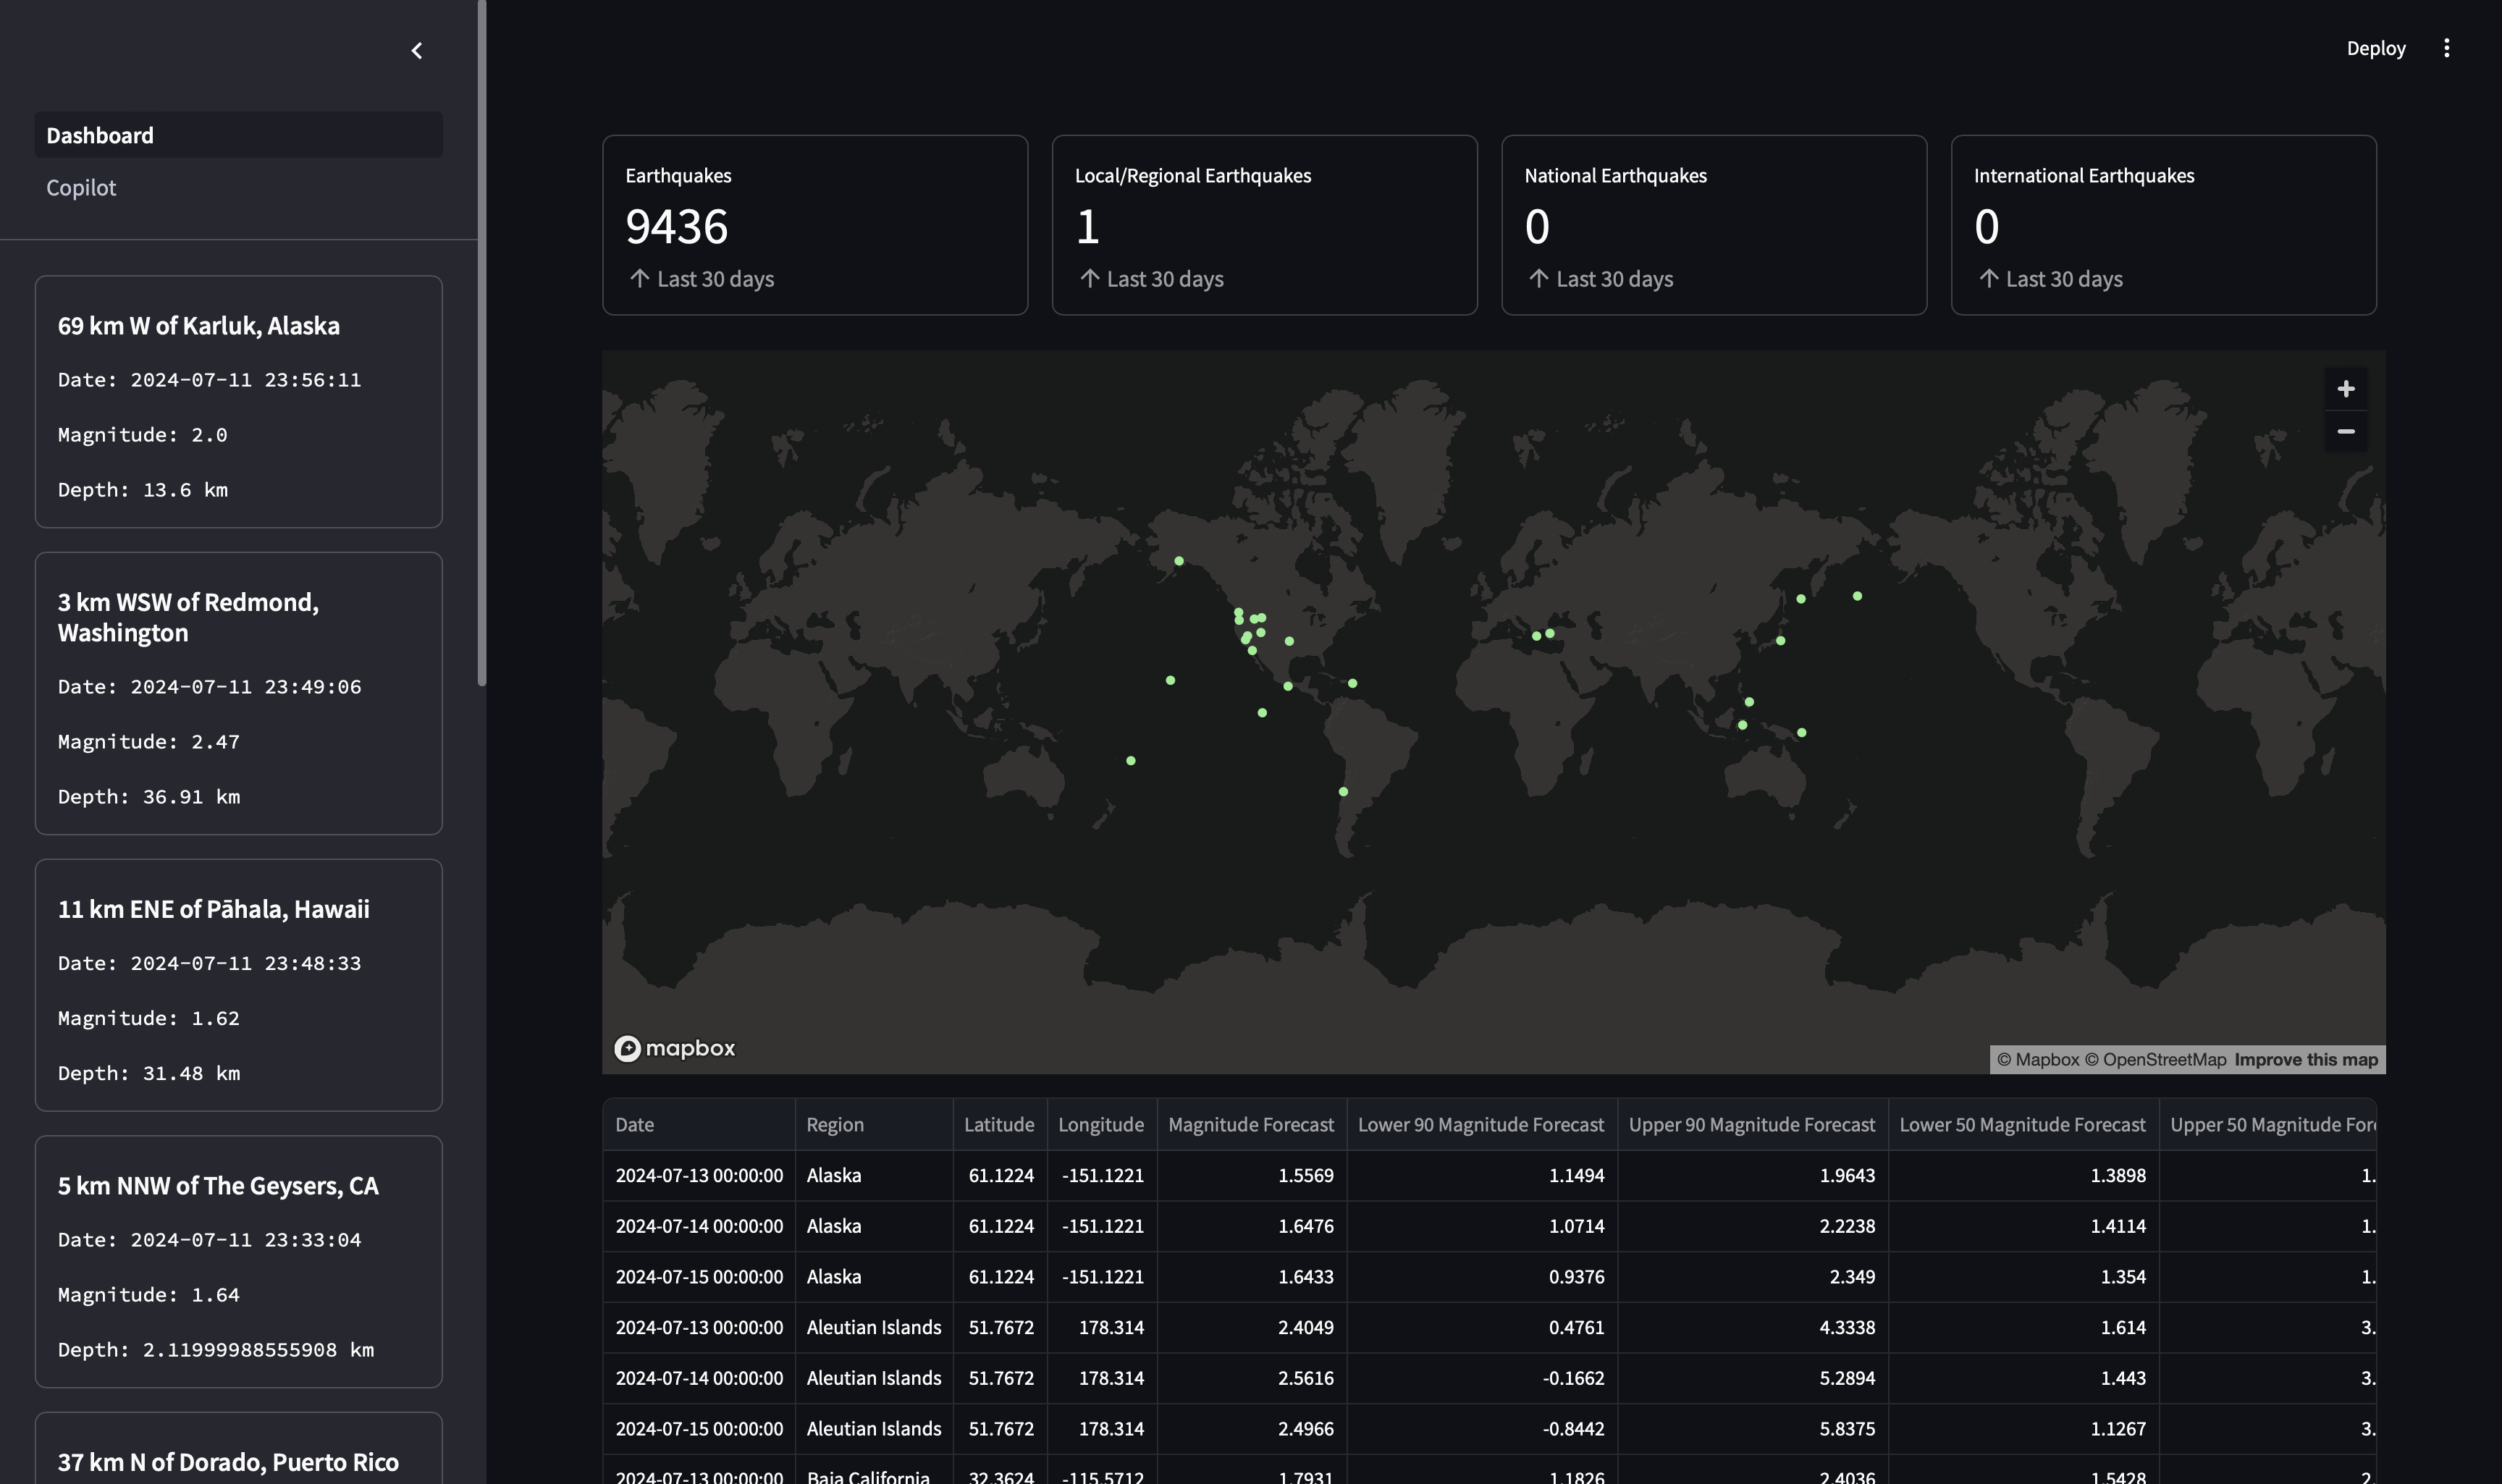
\includegraphics[scale=0.2]{img/dashboard.png}
%       \captionsetup{format=hang}
%       \caption{\label{fig:autogen}Diverse \ac{llm}-based applications
%             using multi-agent conversations. (Left) Customizable agents that
%             can be based on \acp{llm}, tools, humans, or a
%             combination of them. (Top-middle) Agents can converse to solve tasks.
%             (Right) Chatbot, potentially with humans in the loop.
%             (Bottom-middle) Flexible conversation patterns.}
% \end{figure}

% \begin{figure}[h]
%       \centering
%       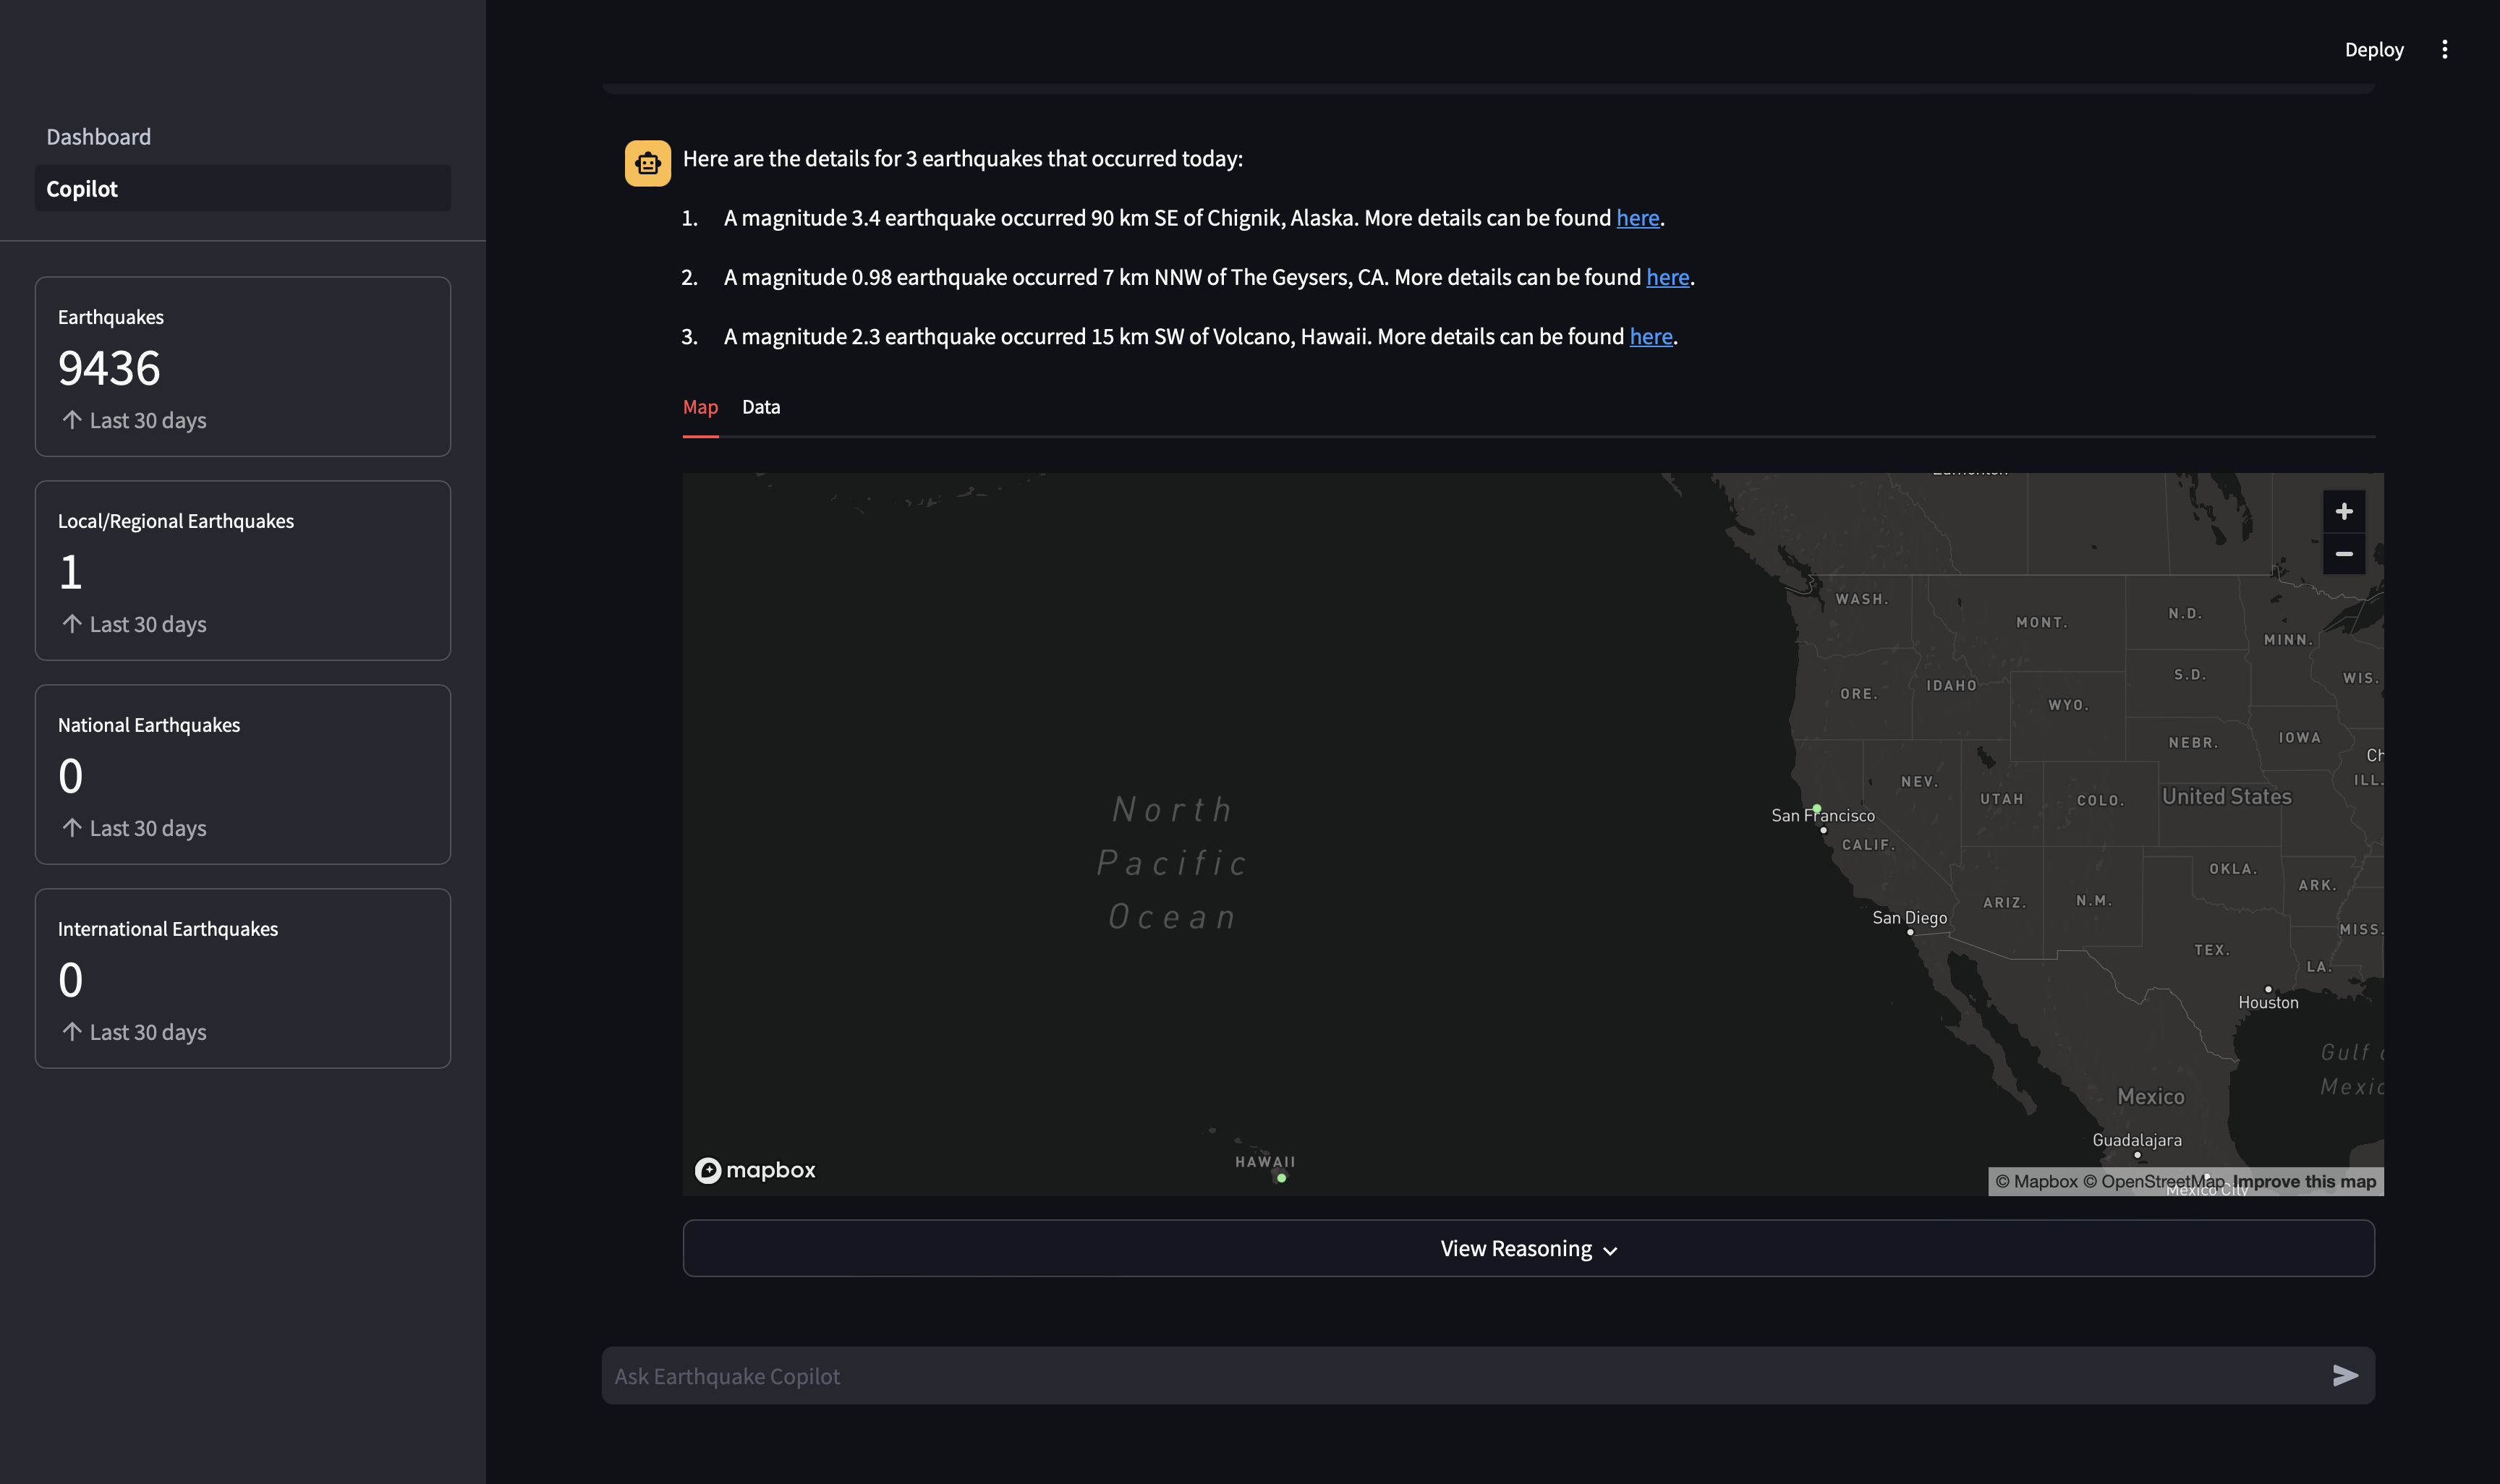
\includegraphics[scale=0.2]{img/llm-powered-ai-agent.png}
%       \captionsetup{format=hang}
%       \caption{\label{fig:autogen}Diverse \ac{llm}-based applications
%             using multi-agent conversations. (Left) Customizable agents that
%             can be based on \acp{llm}, tools, humans, or a
%             combination of them. (Top-middle) Agents can converse to solve tasks.
%             (Right) Chatbot, potentially with humans in the loop.
%             (Bottom-middle) Flexible conversation patterns.}
% \end{figure}

% talk about explainable ai agent somewhere with react prompting we can show the user what the LLM is actually doing behind the scenes, e.g. thought, tool, tool input, tool response, ... thought, final answer to build trust and transparency with LLMs

% \begin{figure}[h]
%       \centering
%       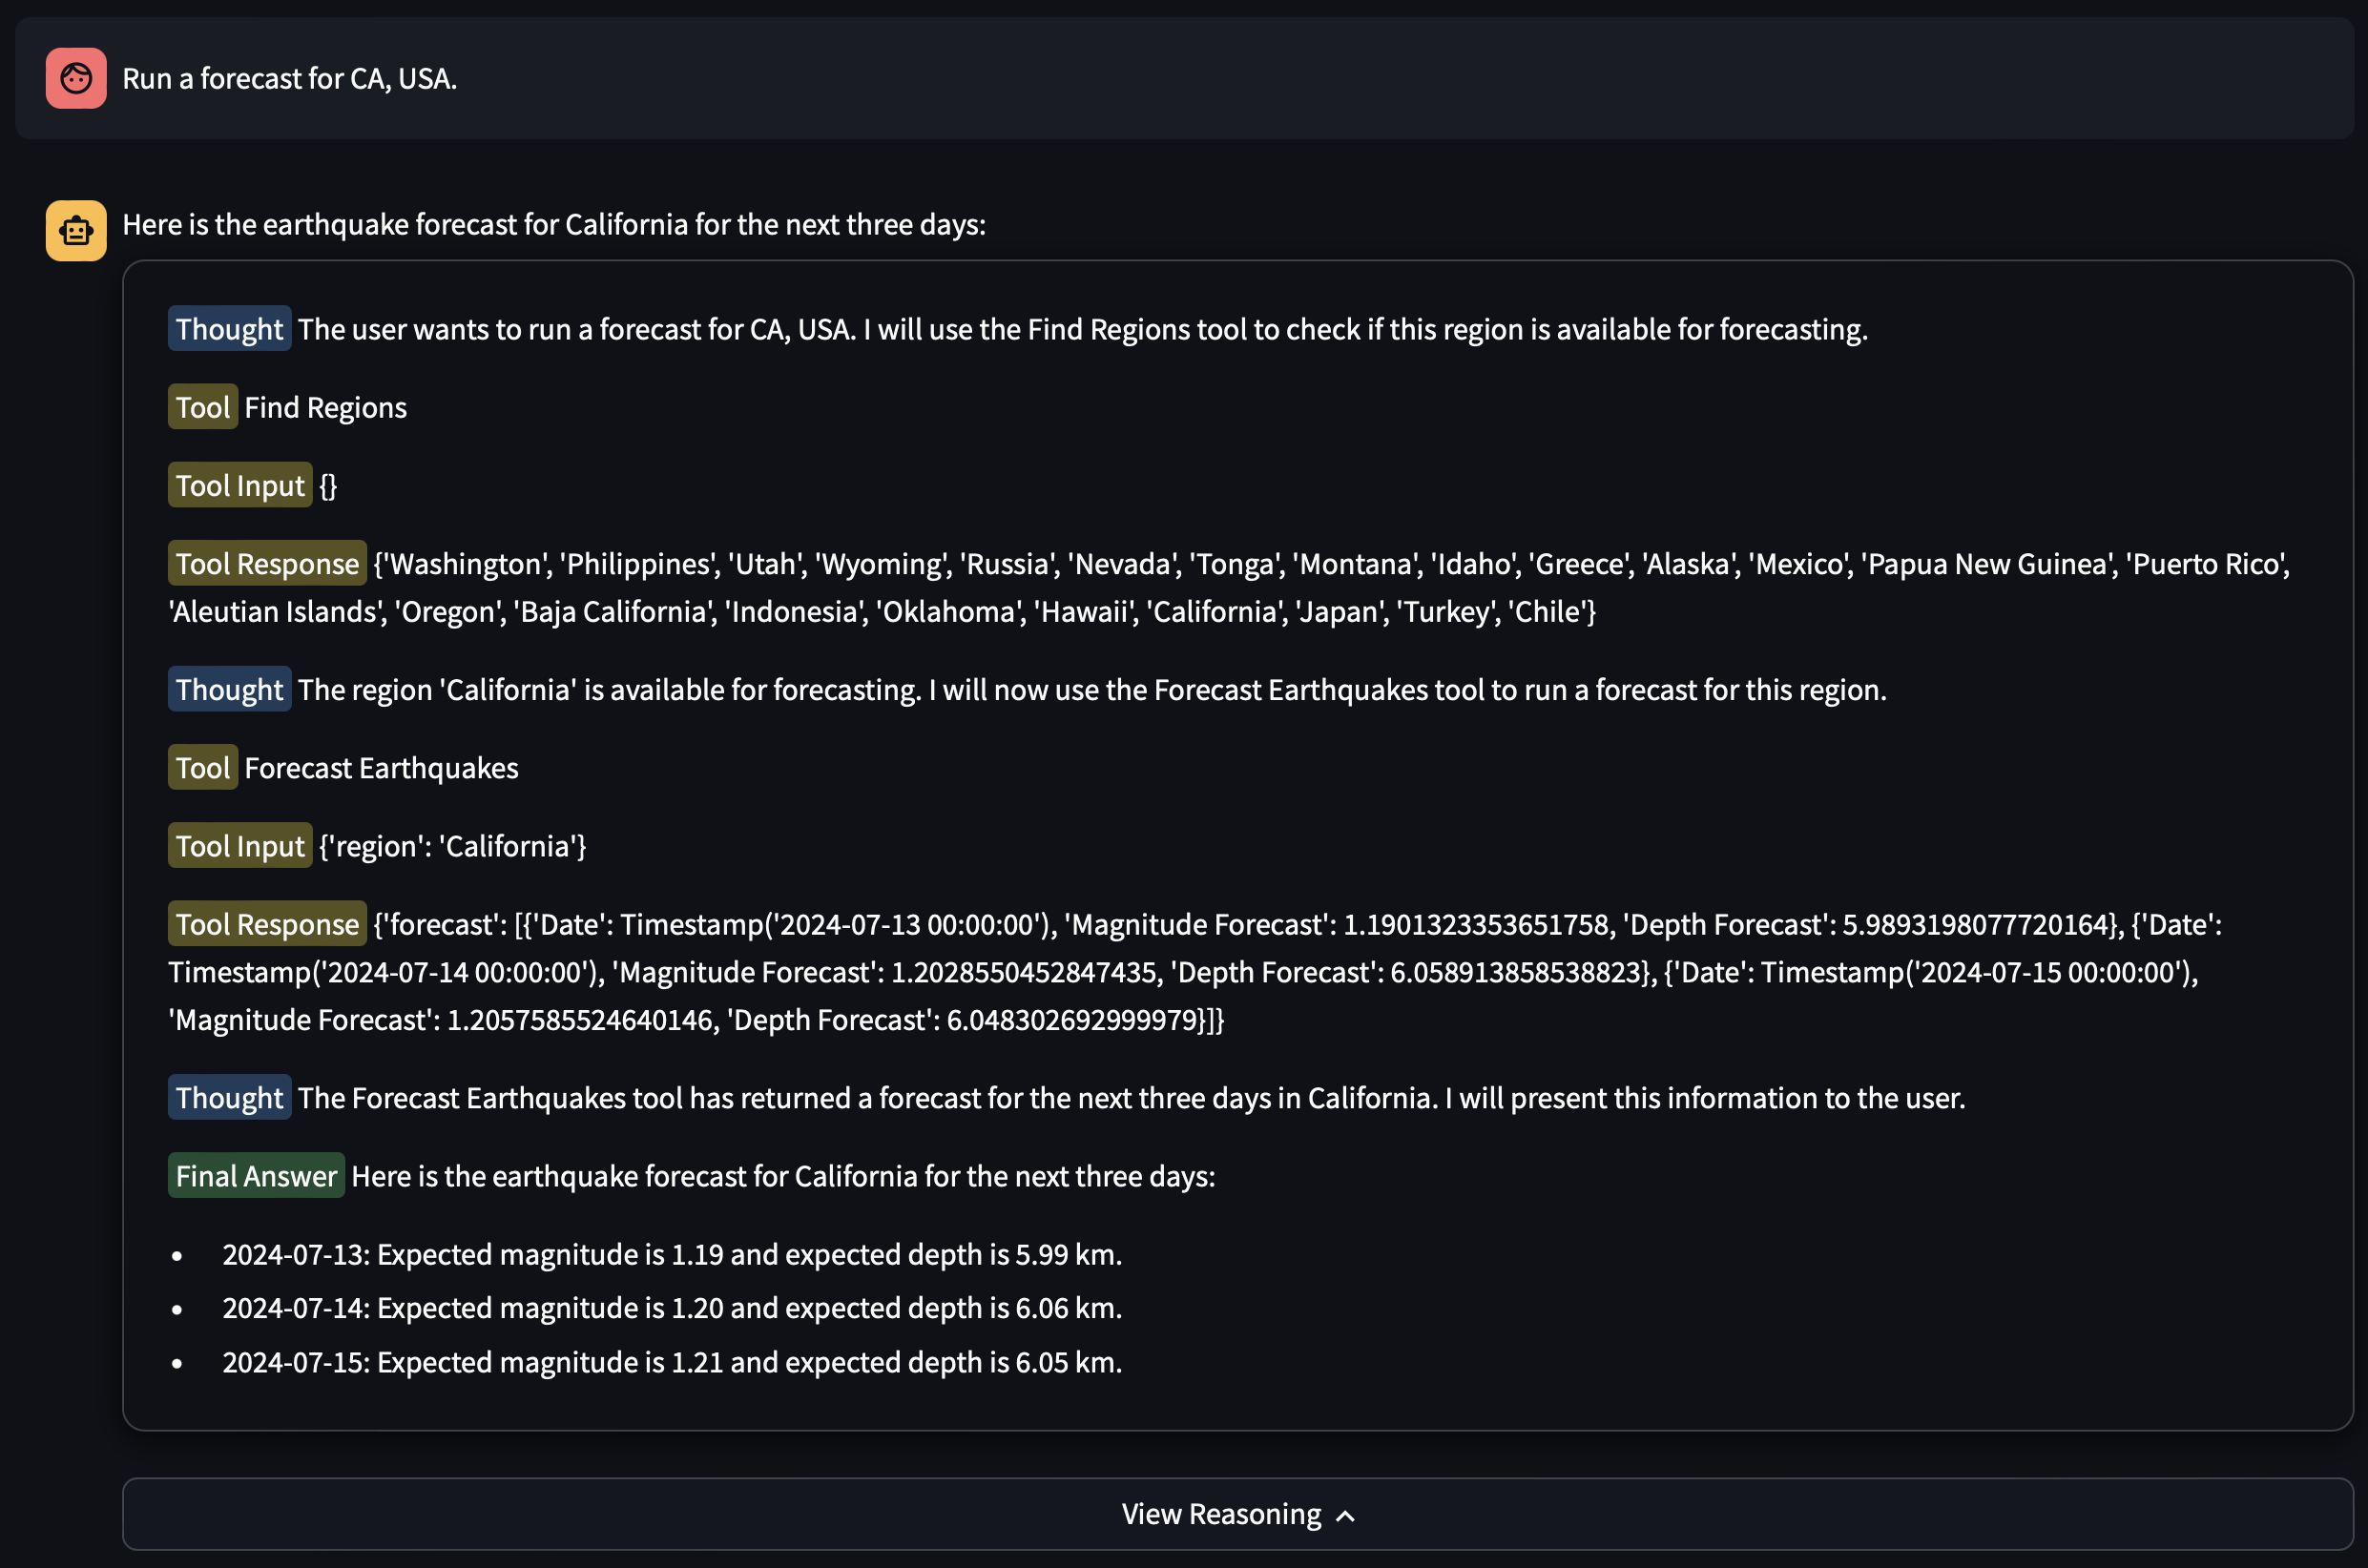
\includegraphics[scale=0.375]{img/explainable-ai-agent.png}
%       \captionsetup{format=hang}
%       \caption{\label{fig:autogen}Diverse \ac{llm}-based applications
%             using multi-agent conversations. (Left) Customizable agents that
%             can be based on \acp{llm}, tools, humans, or a
%             combination of them. (Top-middle) Agents can converse to solve tasks.
%             (Right) Chatbot, potentially with humans in the loop.
%             (Bottom-middle) Flexible conversation patterns.}
% \end{figure}

\section{Deployment and Monitoring}
The first step in deploying our ML application involved containerizing the model using Docker\footnote{\url{https://www.docker.com/}}. Docker allowed us to package the model along with its dependencies into a container, ensuring consistency across different deployment environments. After saving the model, we created the Dockerfile and the Docker Image to install dependencies and run the code.

For deploying the Flight Base App on Render.com, the team optimally utilized the platform's versatile features. Render.com uses Amazon Web Services (AWS) under the hood, which provided the team with a solid infrastructure and worldwide availability through the AWS data center in Frankfurt. The app deployment is automatic as soon as changes are pushed to the team's GitHub repository and the deployment branch is synchronized.

To handle the model's computational demands, especially for real-time predictions, deploying the Docker container on a cluster with GPU support would be ideal. Although we did not have access to a GPU-supported cluster for this project, it is a practical approach when high performance is needed. The deployment would typically be managed through a fully orchestrated workflow. In practice, the training and deployment workflow are fully automated, which can be implemented using Argo Workflows\footnote{\url{https://argoproj.github.io/workflows/}}. However, this was out of scope for this project.

Additionally, when deploying models in practice, using a platform like Kubeflow\footnote{\url{https://www.kubeflow.org/}} is beneficial. Kubeflow leverages Kubernetes for machine learning and allows you to write templates defining how to deploy models, specifying resources such as RAM, CPU, and GPU, as well as managing canary rollouts and other deployment strategies.

The management of environment variables is handled directly through Render.com. These are automatically inserted during the build of the Docker container and are available to the application. Through this approach, the team ensured that the entire deployment configuration remains clear and efficient, while also ensuring a smooth live deployment of the application on Render.com. This method minimizes the risk of misconfigurations and simplifies the management of sensitive data such as API keys.

Furthermore, effective monitoring of the deployed model is crucial to ensure that it continues to perform as expected. Our monitoring process includes checking for model drift, both data drift and concept drift. Model drift occurs when the statistical properties of the target variable (concept drift) or the input features (data drift) change over time, leading to a decline in model performance. An example for a concept drift in earthquake forecasting would be a change in the relationship between seismic precursor signals (like foreshocks, ground deformation, or gas emissions) and the occurrence of an earthquake due to new geological activities or shifts in tectonic plate interactions. Data drifts would include a change in sensor calibration, which would lead to a shift in the data they collect. Additionally, the performance metrics of the model on live data are monitored. Consequently, the model is retrained if the performance metrics decline below a certain threshhold.

In summary, while this project did not employ advanced orchestration tools or GPU-supported clusters due to constraints, these are critical considerations for deploying robust and scalable machine learning models in a production environment.


% Fazit und Ausblick
% !TEX root =  master.tex
\chapter{Conclusion}\label{ch:conclusion}
To conclude, the project was successfully completed, and its goals were achieved.
We preprocessed the data and trained a robust model, which was then used to build a
comprehensive application. This application features a dashboard displaying recent
earthquakes and an interactive map showing future earthquakes for the next three days
worldwide. Given the extensive volume of the presented data, which might seem overwhelming,
we developed an AI agent to increase accessibility. This agent allows users to run
personalized forecasts tailored to their specific needs. Since most users are
interested in one or two regions rather than all 25 regions covered by the forecast,
this feature is particularly useful. Additionally, the AI agent acts as a \ac{USGS} expert,
providing users with in-depth analysis on potential risks and safety precautions for individual earthquakes.

Recognizing that many people are not tech-savvy and aiming to spread information
about earthquakes to a broad audience, we minimized technical barriers. By integrating
an interactive AI agent, we made it easier for users to access and understand crucial
earthquake information.

To enhance the predictive accuracy of earthquake forecasting models, several potential
improvements can be considered. Integrating live data such as magma flow, plate tectonics
movements, and real-time seismic activity could provide a more comprehensive and dynamic
understanding of the underlying processes that precede earthquakes. Additionally, exploring
advanced deep learning models, such as \ac{RNNs} and \ac{LSTM}s, which are well-suited for time series
data, might offer improved prediction capabilities by capturing complex temporal dependencies.
Furthermore, incorporating multi-source data fusion techniques, which combine various types of
geological and environmental data, could enhance the robustness of the model. Continuous
updates and retraining of the model with the latest data, along with cross-disciplinary
collaboration between seismologists and data scientists, would also contribute to refining
the forecasting accuracy.

However, it is important to acknowledge the inherent unpredictability of earthquakes.
Similar to predicting stock market values, earthquakes are fundamentally random and
complex events, making precise forecasting exceptionally difficult. Despite robust
statistical models, accurate predictions remain elusive. Nonetheless, these improvements
could collectively aid in better anticipating seismic events despite their chaotic nature.
%%%%%%%%%%%%%%%%%%%%%%%%%%%%%%%%%%%

%%%%%%%%%%%%%%%%%%%%%%%%%%%%%%%%%%%
% ANHÄNGE
%
% @stud: einzelne Anhänge bearbeiten und eigene Anhänge hier einfügen
%        die nachfolgenden Zeilen deaktivieren, wenn keine Anhänge verwendet werden
%
\initializeAppendix
% !TEX root =  master.tex
\chapter{Web Application Design}\label{ch:web-application-design}

\begin{figure}[hbtp]
    \centering
    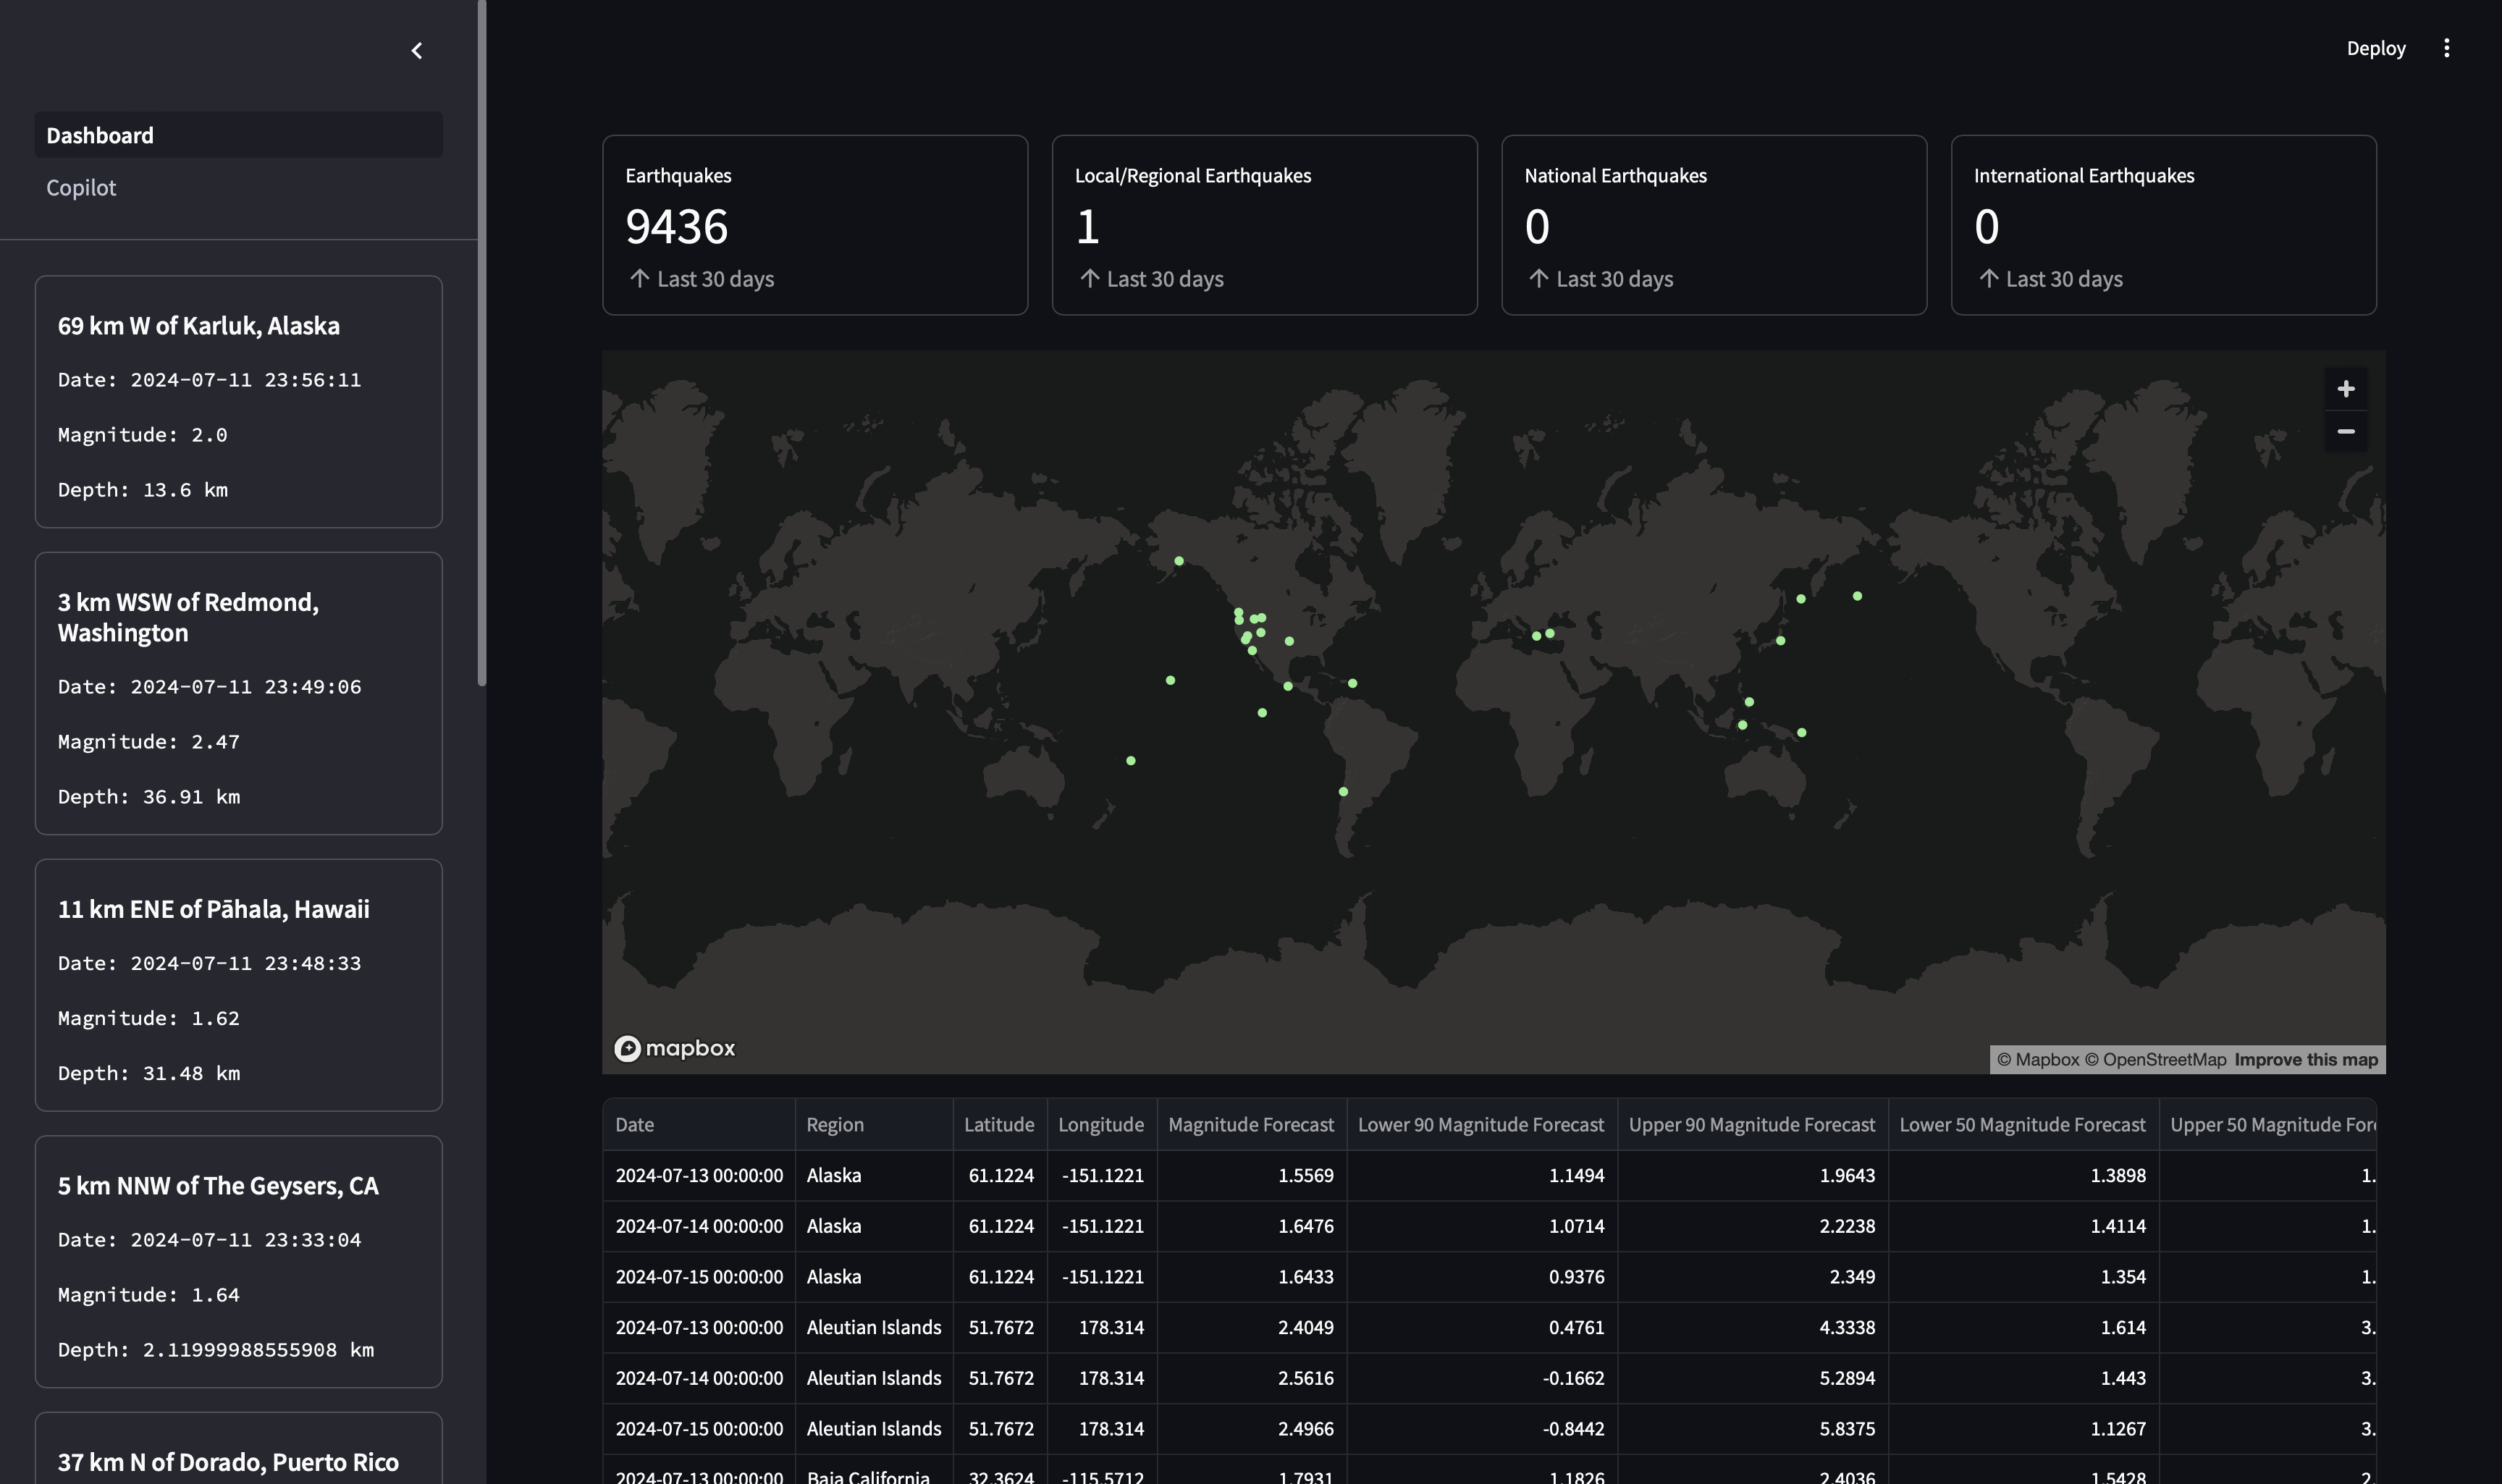
\includegraphics[scale=0.25]{img/dashboard.png}
    \captionsetup{format=hang}
    \caption{\label{fig:dashboard}Interactive dashboard displaying
        recent earthquakes, with a map featuring earthquake forecasts
        and a corresponding table detailing the forecasted values for
        magnitude and depth.}
\end{figure}

\begin{figure}[hbtp]
    \centering
    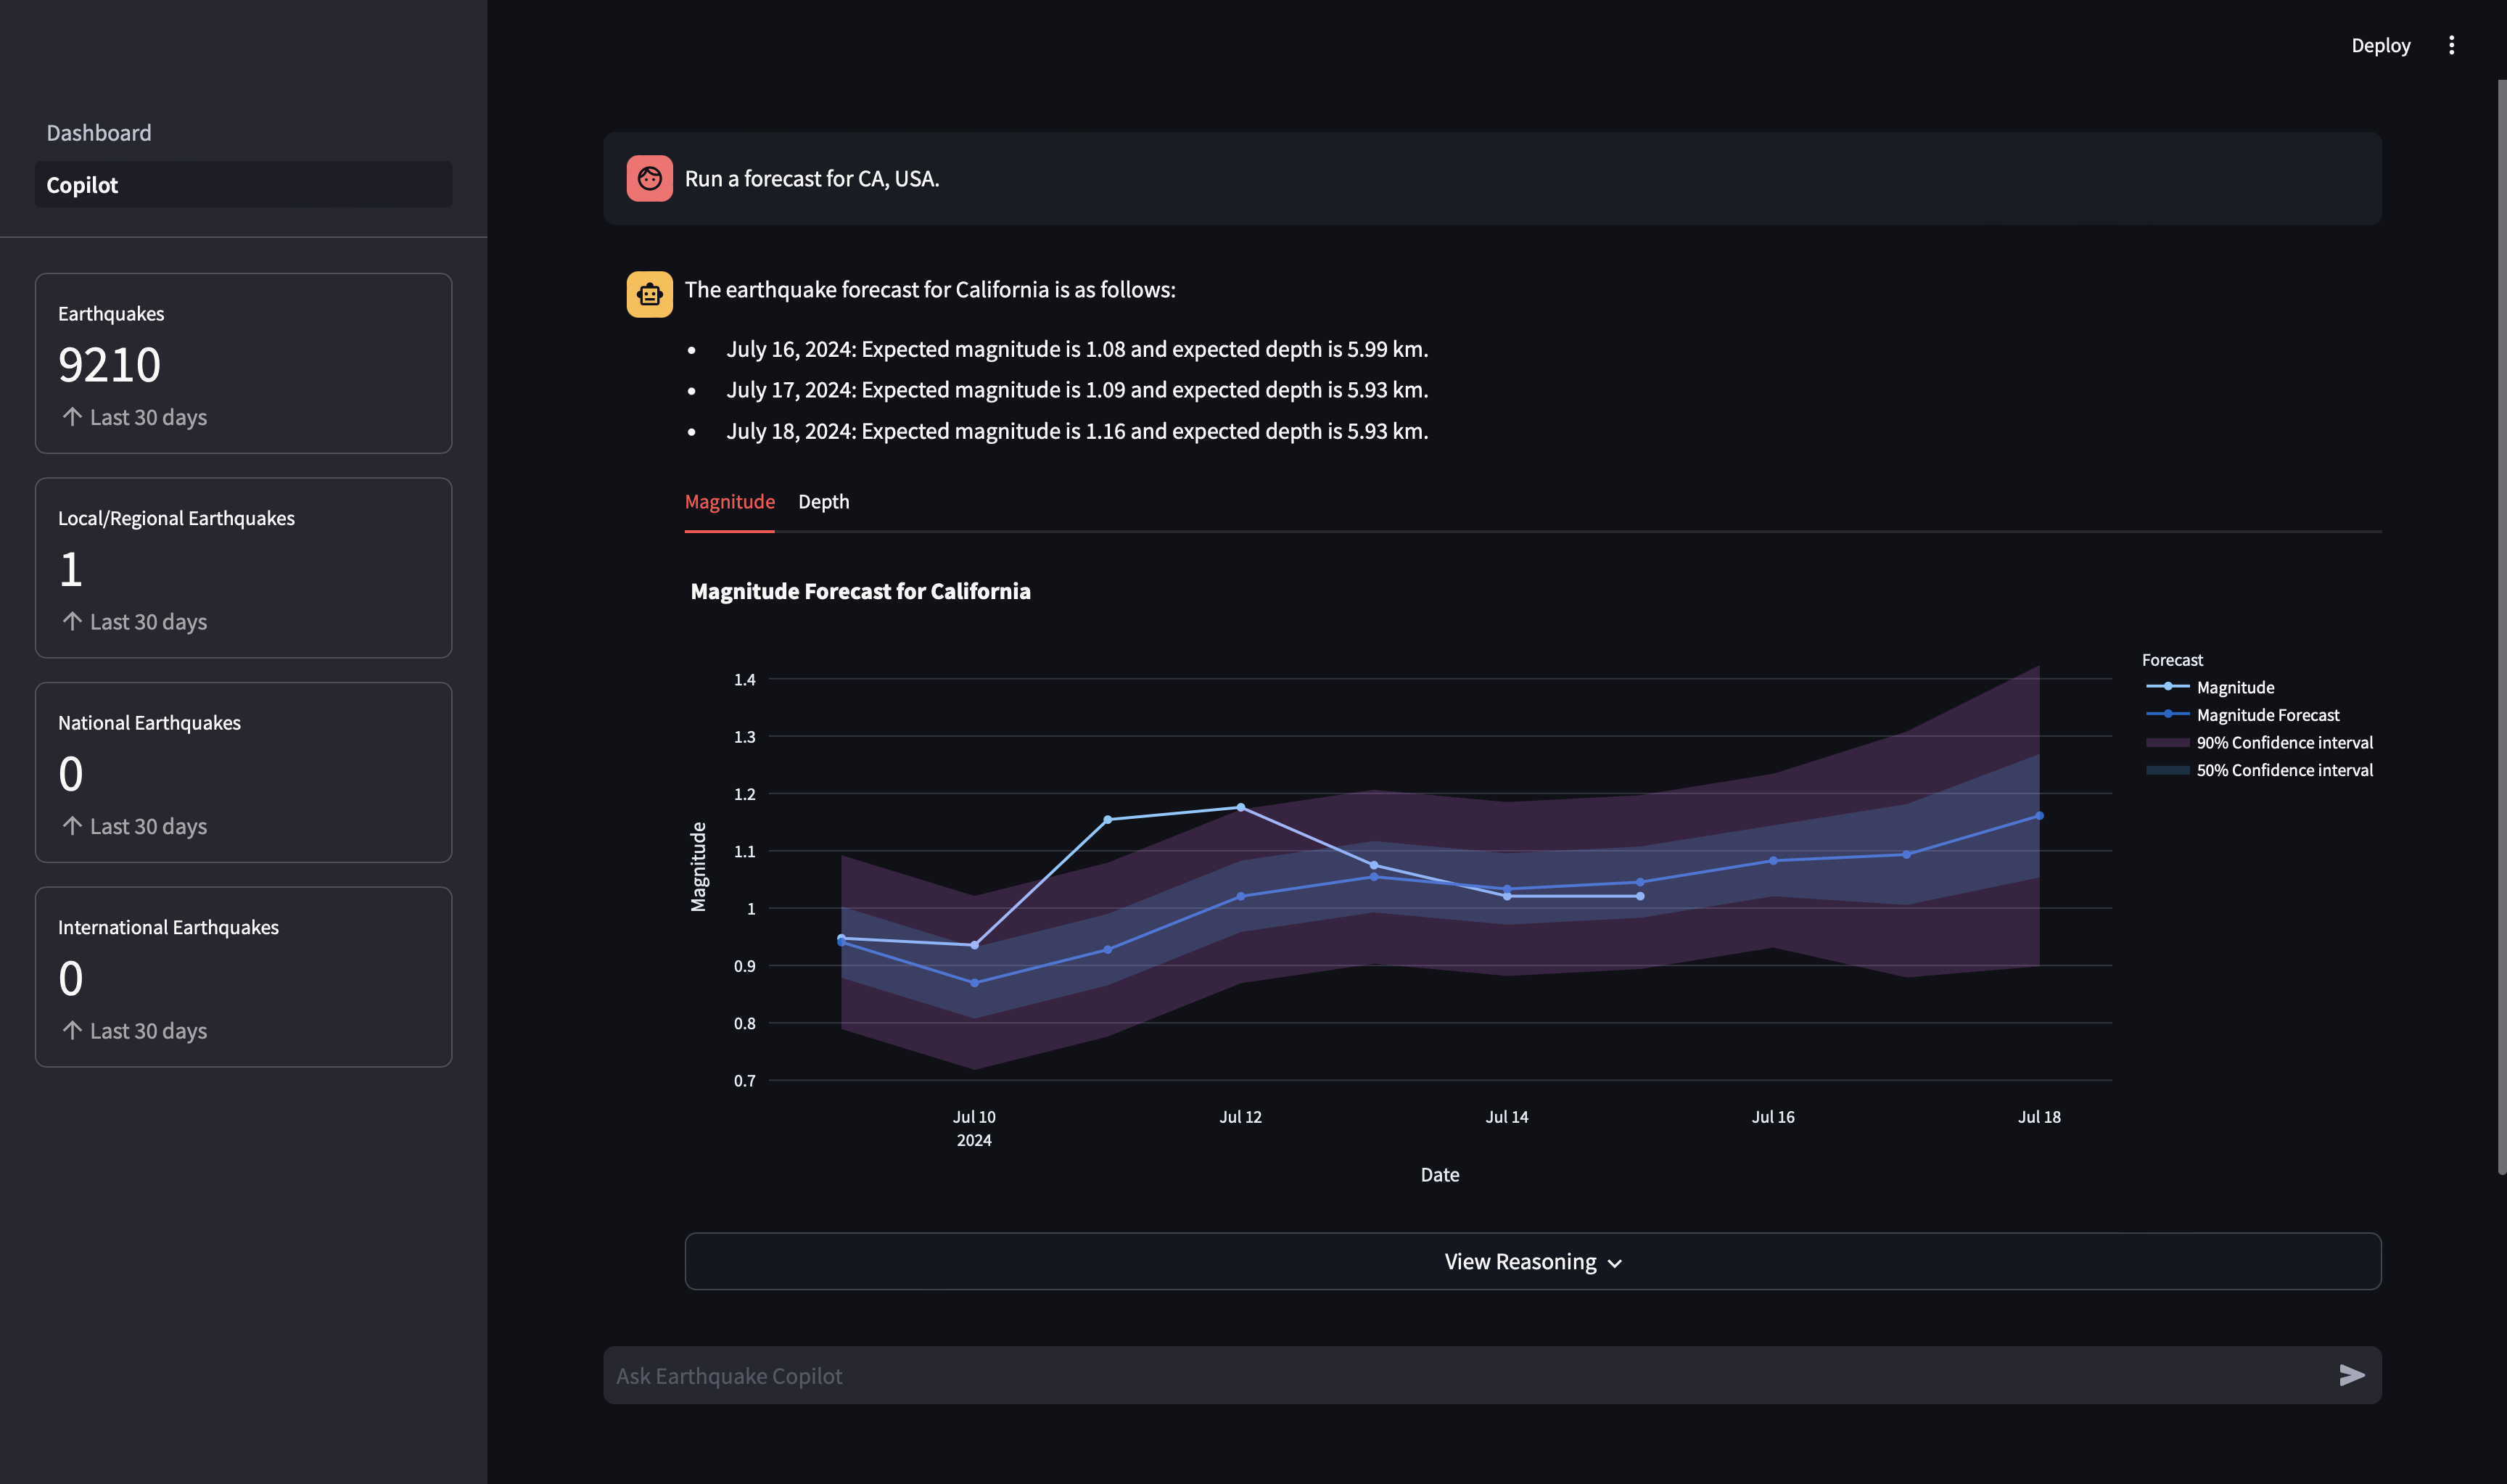
\includegraphics[scale=0.25]{img/copilot-forecast-example.png}
    \captionsetup{format=hang}
    \caption{\label{fig:copilot}Copilot interface showcasing human-AI
        collaboration, where an \ac{LLM}-powered AI agent assists by
        answering questions, running forecasts, and recommending
        precautionary actions.}
\end{figure}

\begin{figure}[hbtp]
    \centering
    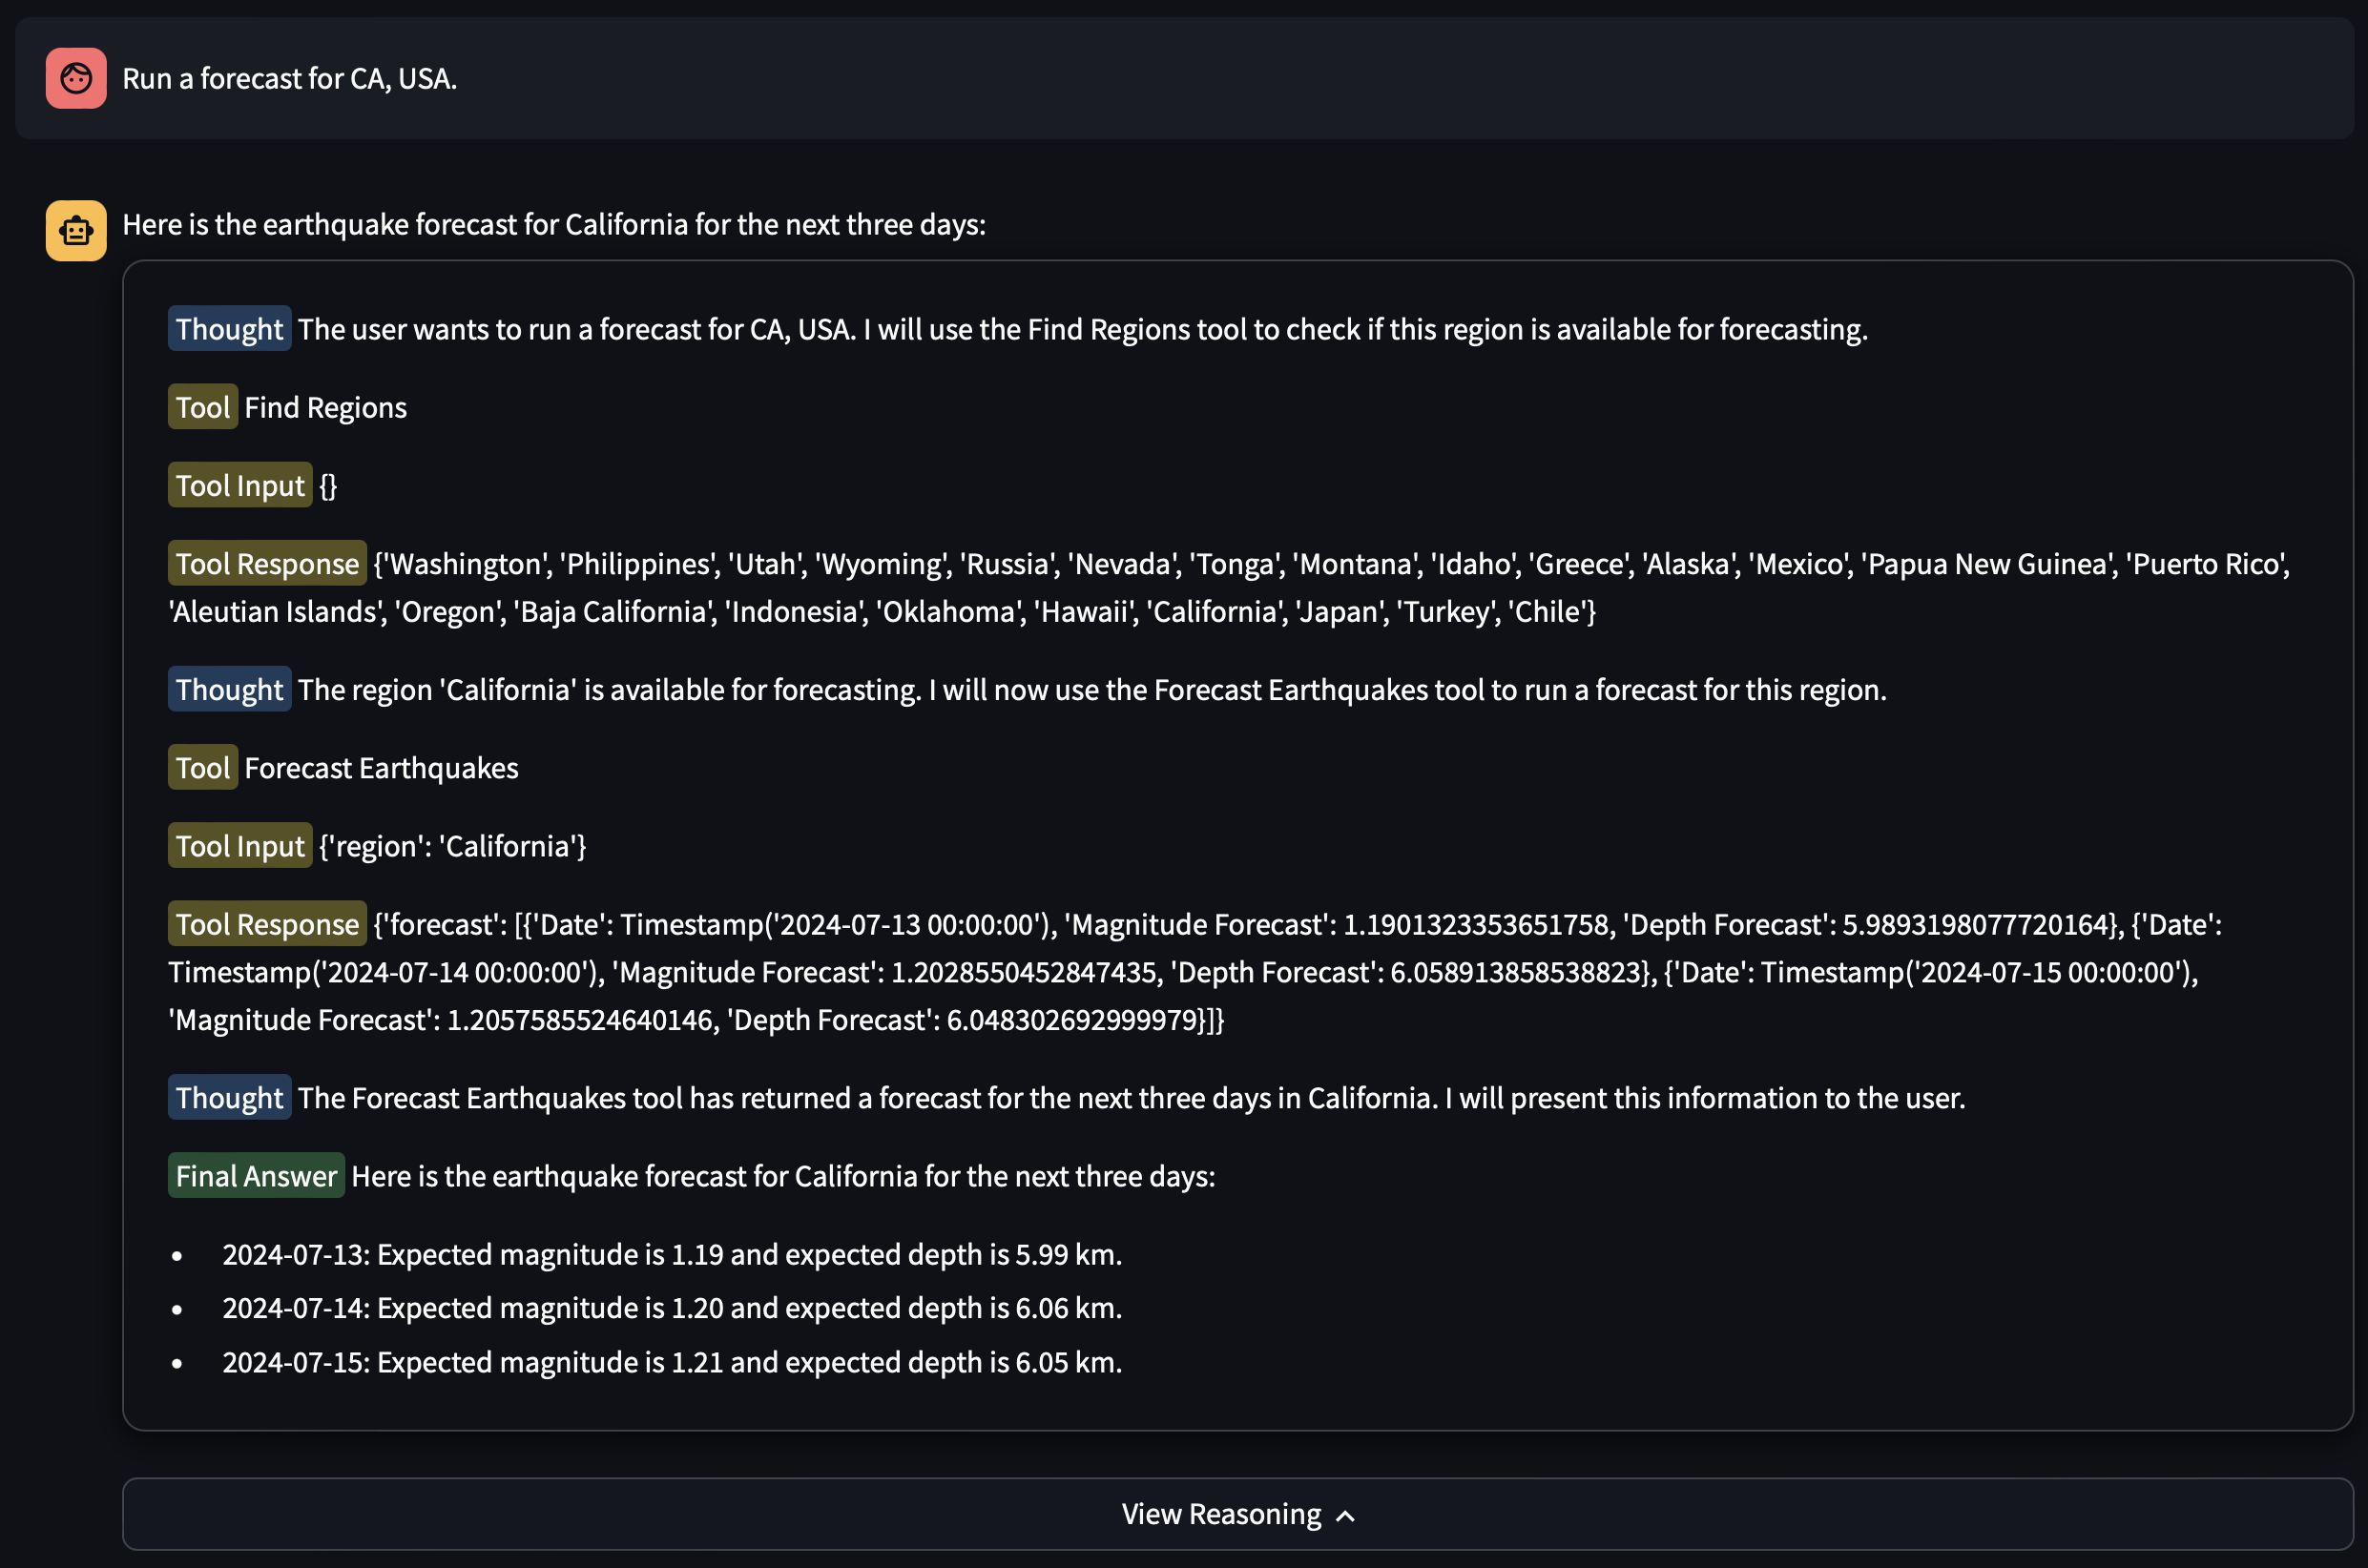
\includegraphics[scale=0.35]{img/explainable-ai-agent.png}
    \captionsetup{format=hang}
    \caption{\label{fig:explainable-ai}Explainable AI in action:
        The \ac{LLM}-powered AI agent demonstrates its reasoning process as
        it runs a forecast for California, USA. By following the
        reasoning steps, the user can verify the accuracy and
        transparency of the \ac{LLM}'s operations, thereby building trust.}
\end{figure}


% !TEX root =  master.tex
\chapter{Beispiel-Anhang: Noch ein Testanhang}
nochmal: lipsum ...

%%%%%%%%%%%%%%%%%%%%%%%%%%%%%%%%%%%

\singlespacing

%\ihead{}
%\printbibliography[title=\Literaturverzeichnis]
\printbibliography
\cleardoublepage

%\initializeBibliography
%%%%%%%%%%%%%%%%%%%%%%%%%%%%%%%%%%%

%%%%%%%%%%%%%%%%%%%%%%%%%%%%%%%%%%%
% INDEX
% @stud: ggf. Index auskommentieren, wenn nicht benötigt
%
% \addcontentsline{toc}{chapter}{Index}
% \printindex

\end{document}
